% Created 2023-06-30 Fri 08:50
% Intended LaTeX compiler: pdflatex
\documentclass[11pt]{article}
\usepackage[utf8]{inputenc}
\usepackage[T1]{fontenc}
\usepackage{graphicx}
\usepackage{grffile}
\usepackage{longtable}
\usepackage{wrapfig}
\usepackage{rotating}
\usepackage[normalem]{ulem}
\usepackage{amsmath}
\usepackage{textcomp}
\usepackage{amssymb}
\usepackage{capt-of}
\usepackage{hyperref}
\author{Filipa  Calado}
\date{\today}
\title{}
\hypersetup{
 pdfauthor={Filipa  Calado},
 pdftitle={},
 pdfkeywords={},
 pdfsubject={},
 pdfcreator={Emacs 26.2 (Org mode 9.1.9)}, 
 pdflang={English}}
\begin{document}

\tableofcontents

\section{new draft}
\label{sec:org5e0f692}

\subsection{hook}
\label{sec:org97695f1}

[[/images/desire.png][The desire to write is the desire to fool you, seduce you. Here I am -
again - always getting the girl, saying the right thing or (toss this
in for effect) something deliciously, winsomely wrong. Look over there
\begin{itemize}
\item that's me, at four\ldots{}]]
\end{itemize}

Caitlin Fisher's electronic work, \emph{These Waves of Girls}, guides the
reader through the story's various interconnected episodes with
hyperlinks attached to seductive phrases like "the desire" or "that's
me, at four\ldots{}" to link one page to another
("desire\(_{\text{to}}\)\(_{\text{write.htm}}\)"). These links connect and support this works
associative structure while also tempting the reader to traverse (by
clicking through) the story, which is an autobiographical account of
the author's sexual coming-of-age.

Though they are an associative tool, the hyperlinks that connect one
page to the next frustrate the sense of narrative coherence across
this text. The number of links presents what James Pope describes as
"a baffling range of choices for movement which actually led to a
stifling of movement altogether" ("Significance"). The profusion of
these links offers too many narrative paths that disrupt the
relationship between cause and effect in the story, scrambling the
reader's sense of progress as she traverses the text.

Not only do the links inform the narrative coherence, they also play
on the reader's desire. In addition to pursuing a continually deferred
sense of narrative closure, the reader also chases a elusive
understanding of the narrator's sexual discovery, of which the reader
only ever gets part of the story. For example, 

For example, one repeatedly linked page displays words "and it was the
most erotic year of my life" march across the screen like ticker tape
is accessed from two separate points ("And it was…") 

[GIF EROTIC TICKER TAPE]

This disseration begins with a conviction that digital media and
queerness share a preoccupation with a kind of frustrated
sensuality. One way this emerges is through the sense of touch, the
desire for touch, and its disappointment. Touch and its frustration is
figured quite literally in an electronic work by 

This node is accessed from two different pages that relate very
different stories. The first access point comes from the “beam
routine” episode, tells a story about the 15-year-old narrator,
Tracey, and her close friend, Vivian, coaxing older men to buy them
drinks at a bar ("warned.htm"). The narration interweaves the central
action, which is the girls’ efforts to get attention from the adult
men at the bar, with moments of intimacy between the girls. Tracey
narrates that “Our third daiquiris arrive and, my hand hot on her
waist, I tell her I love her. She loves me too, she says, just not as
much as I love her” (“beamroutine5.htm”). After a few more drinks,
Tracey goes into a hotel room with an older man, "the shoe-salesman,"
where the following scene ensues: 
\begin{quote}
‘I don’t want to have sex,’ I say. ‘Not with you.’

But then, not wanting to disappoint, ‘I could do my beam routine.’  

I take off my clothes and, fifteen, mount the line of the carpet to
perform my entire junior beam routine, handstand press, two
backhandsprings included. He jerks off. Dismount.  

I hurry into my clothes and head home to Vivian (who loves me, but not
as much as I love her). For years I worry that the shoe salesman was
really disappointed, stuck with a fifteen year old virgin gymnast
rather than a real bad girl. "Beamroutine8.htm"
\end{quote}
From this small excerpt, we can note a couple of crucial elements of
the larger narrative. First is the instability or elusive nature of
desire. Here, when the narrator says, “not with you,” she implies that
the intended target of her desire may be Vivian, rather than the shoe
salesman. The moving target of the narrator’s desire will prove to be
a difficult one to follow as the story progresses. 

The second point is the tension between sight and touch. The beam
routine performance, while compensating for the sexual act that Tracey
withholds from the shoe salesmen, also literalizes the modality of her
desire. It is a performance which is accessed by sight rather than
touch. It is interesting that this medium makes the story accessible
through touch (the “click” on the hyperlinks) while not giving full
visual access to the individual narratives like a traditional print
work (which is a phenomenon exaggerated in the ticker tape). In other
words, the tension between sight and touch for the reader in accessing
the story mirrors the cycles of desire and frustration within the
story world. The hyperlinks seduce and draw the reader to click
through to new parts of the story, parts which can frustrate our grasp
of the story as a whole.

As the reader familiarizes herself with the events of the story, she
is always losing context. The link to “He jerks off” leads to another
page, aptly titled “erotic,” where the phrase “and it was the most
erotic year of my life” marches across the screen like ticker
tape. This “erotic” page can be accessed from (at least) two different
narrative paths, both featuring sexual episodes between the narrator
and men. In a story that mostly focuses on self-described “lesbian’
desire, the association between eroticism and men creates a sense of
dissonance, which is reinforced by another, inverse association,
between women and lack of sexual desire. On this same page, the phrase
“I don’t want to have sex” leads to an often-linked node about Jennie
Winchester, the narrator’s “grade 11 girlfriend” (“want.htm”). This
node details the following episode:
\begin{source}
I’m in bed with Jennie Winchester and I realize she wants me to undo
her pants. She needs to be home by 11:00 and needs to leave my place
by 10:45. I’m kissing her but opening my eyes at intervals to catch
the clock. At exactly 10:43 I unbutton her Levis and shove my hand
inside, barely undoing the zipper. “I’m in bed…”
\end{source}
This node, and the others which depict Jennie, presents her as a
highly desirable sexual partner. However, by following the previous
link, the reader experiences this familiar node from a new narrative
path, originating from “I don’t want to have sex.” By sharing nodes
like this, many of the potential pathways in this text interweave to
complicate our understanding of the narrator’s sexual desire,
presenting sexuality as something elusive or difficult to pin
down. Now the reader experiences this familiar node in a new way that
casts its former meaning into doubt. What is the connection between
this episode and the phrase, "I don't want to have sex"? Why is the
narrator watching the clock? Because the character's desires have been
muddled by the unpredictable connections between episodes, what at
first seems straightforward now appears to support alternate
readings. The reader’s confusion in navigating through Waves, in
re-interpreting fragments that had been previously integrated,
reinforces queer identity as something elusive, a condition that is
not fully intelligible. Clicking (touching) her way through the
narrative, the reader is repeatedly reminded of her removal from the
distance from the narrator.

Associations between the digital and touch expand from numerical
computation (the ten "digits" of the hand) to the haptic connections
made through the intermediaries of mice, keyboards, and eventually,
touch screens. These intermediaries demonstrate that humans engage
with electronic data at a remove, through layers of computation and
abstraction, which paradoxically puts them into direct contact. 



\section{old draft}
\label{sec:org6c9cbb0}

\subsubsection{revision notes}
\label{sec:org2b38d4c}
\begin{enumerate}
\item chapter summary
\label{sec:orge4df156}
This dissertation looks at new ways of reading \emph{queer bodies} and
\emph{queer subjectivity} within technological contexts. How do digital
tools and platforms change the way we interact with queer
subjects/affects/embodiments within texts? What about the digital
allows us to activate \emph{sensational} reading experiences? In simpler
words, how does digital media interface with queerness?

This chapter proposes a reading methodology that leverages the
critic's relationship to the text to open possibilities for
interpretation and connections to the textual material. It explores
the ways that reading practices across two different fields (digital
humanities and queer theory) intertwine, and how this creates a new
method for reading queer narratives in digital contexts.

First, queerness is established as something that can only be touched
"at a distance," because the queer subject cannot be redeemed or
recovered. This impulse to satisfy, redeem, or recover queerness is
observed in “paranoid” or “suspicious” reading practices, which seek
to answer or discover the “hidden” meaning within text. These
practices attempt to answer questions, but do so in a way that
constrains inquiry, because paranoia only delivers the results that
are \emph{imaginable} within current the knowledge structures. To avoid
reproducing these knowledge structures, we must look to strategies
that do not assume full connections, look to queer affects, like
\emph{queerness as not yet here}, \emph{touching/feeling}, \emph{feeling
backward}. We value abstraction, or \emph{queer form}, which is necessary
for bringing things into relation, and opacity, which keeps the
unknowable nature of queer experience and identity somewhat in
tact. We look at \emph{Confessions of the Fox}, \emph{These Waves of Girls},
\emph{Borderlands}.

The history of computing and media shows how tools were built in ways
that are not neutral, and we find DH practitioners doing work that is
critical of digital methods. Looking at the example of DH from the
position of queerness we see more clearly the necessity of opacity,
formalization, and abstraction as reading methods, and the real danger
of reproducibility and totalization, byproducts of paranoia. We find
parallels between queer critics and feminist DHers, who are doing
something similar; we interweave Saidiya Hartman and Lauren Klein.

Finally, we propose three values for queer DH, which is: novelty (the
performative), vantages (the visual), and provisionality (the
ontological). We see these examples in \emph{these waves of girls}, and
\emph{the confessions of the fox}.

\item feedback on intro from diss workshop
\label{sec:orgc92657c}
The three heavy footnotes in the beginning, are tripping people up, a
bit overwhelming. Work on spreading this out. In doing so, luxuriate
in the idea of how digital etymology relates to the idea of touch.

clarify specific terms/concepts: 
\begin{itemize}
\item Who is \textbf{\textbf{Matt Kirschenbaum}}? Characterize him a little bit for
outsiders. Situate myself in relation to him. Also consider taking
out or reducing the footnote on materiality, because it's tripping
people up.
\item Explain why I am choosing this word \textbf{\textbf{formalization}} to describe a
construct. What does this term do that "construct" cannot do?
Another sentence on what I mean here.
\item What Queer theory am I using, at \textbf{\textbf{reconsolidation}}. The
abstraction of the queer subject. (related to the issue of
positioning myself w/ regard to queer theory: The ways that queer
subjectivity is constructed differently in early poststructrualism,
as opposed to affect theory. Affect theory tries to bring the body
back, thinking to Sara Ahmed vs Foucault). In addition to defining
my position/sources, also consider how "queer" can be reclaimed by
those it is meant to oppress (Butler, 'Critically Queer').
\item \textbf{\textbf{the sensual fullness of a lack}}: see butler on beauvoir and
irigaray, two women together as a double lack, in gender
trouble. \emph{When our two lips touch}, Irigaray
\item see how \textbf{\textbf{haptic}} is being deployed in other disciplines.
\item what do I mean by \textbf{\textbf{touch as abstraction}} on page 3? The physical
experience of touch may be an abstraction, or abstracted, but it is
not experienced as such. Jacob: "Touch often registers as painful
immediacy". See Ann Cvetkovitch's writing on Stone Butch Blues.
\item on page 3, I'm making sweeping claims about the \textbf{\textbf{Queer
Subject}}. Is there a single queer subject, a queer subjectivity? Do
the narrators demonstrate this? If so, what is that kind of queer?
\end{itemize}

More broadly: 
\begin{itemize}
\item how does the digital relate to the \textbf{\textbf{body}}? how does it change the
body? how does queerness do this? --> Butler's points about how a
body doesn't come into being until contact in \emph{Bodies that Matter}.
\item what am I doing with \textbf{\textbf{touch more broadly}}? why is this chapter
about touch?
\item emphasize that I'm doing this \textbf{\textbf{new thing}}, this new field. DH can
help us theorize the queer; and queer can help us understand the
Digital.
\item clarify the relationship between \textbf{\textbf{removal, touch, and grasp}}. How
are these distinct?
\end{itemize}

In close readings, \textbf{\textbf{the various registers of touch}} are at odds.  
\begin{itemize}
\item I start the chapter by saying that queer and the digital are related
through touch, then I assert that it is a troubled relationship to
touch. Make it clear at the start that I'm thinking about touch as a
complicated activity/phenomenon, not touch as always making
contact.
\item How the implications of touch are slightly different or opposite to
each other across the close readings. One is frustrated touch and
one touch opens up. Establish the connection between the two.
\item There's a tension between literal touch (touching the text) and
figurative touch (touch as a trope, touch via sight). Emphasize and
distinguish the difference between touch as a figure within the text
and as a means of engaging without the text. Additionally, on the
literal side, how is this touch (clicking through) different from
turning the page?
\item revise the close reading of \emph{waves} to include analysis of the beam
routine. How is touch operating? there is no touch in this scene.
\item the paradox of touch: the untouchable is good --- it is a paradox. 
\begin{itemize}
\item the paradox of touch: touching w/o touching
\end{itemize}
\end{itemize}

Revise close-reading of \emph{Waves}
\begin{itemize}
\item people found it confusing regarding "touch" and doesn't cohere as
nicely as \emph{Confessions} with my chapter argument.
\item emphasize dynamics of the beam routine, the not touching in that
episode paralleling the not touching of \emph{Confessions}.
\item explain clearly the removal between reader and text not only in the
level of narrative form but also in the materiality of the substance
of the story, the codes and computation.
\end{itemize}

More readings:
\begin{itemize}
\item on Munoz --> also think about Raymond Williams, and structures of
feelings which will help you elaborate on emergence.
\item will narratology help me clarify some of the terms on page 6, on the
close readings of \emph{Waves}? Mieke Bal perhaps.
\end{itemize}

\item plan for problem section p
\label{sec:org47aa77e}
\begin{enumerate}
\item Outline of this section:
\label{sec:orgcd8b1e4}

(1) defines queerness as affective--the untouchable; 

(2) explores paranoid reading across disciplines as the failure of
discourse;

(3) explores how criticism needs the body \& affect; 

(4) proposes a solution to "touching w/o touching," distance.

\item (1) queer subjectivity based on affect, the untouchable
\label{sec:org480aa97}

We are building an understanding of queer subjectivity that is based
on affect. In the experience of disidentification (Munoz), there is an
feeling of a choque (Anzaldua), a clash of affects, an embodied
experience. That experience contains an element of the incommensurable
(Schutte), a gap. This gap is what is untouchable about queer
experience (Cvetkovitch). It is an affective experience that exceeds
language and discourse.

We are looking for alternative modes of analysis which allow us to
deal with the incommensurable elements of queerness.

\item (2) paranoid reading
\label{sec:org98d4bb9}

The perspective of paranoia shows us the pitfalls of discursive
methods.      

The perspective of paranoia has analogues in history and science.

We deconstruct methods of reading that try to ascertain truth or
verify facts.

\item (3) criticism needs affect \& embodiment (hesitation)
\label{sec:orge900cc5}

We cannot capture, grasp, or access queerness by discursive means, we
must turn to affect.

We conclude here that the proper position is hesitation, restraint. An
awareness of the need for hesitation, while also embracing
embodiment. The challenge is to regain touch without resolving it.

\item (4) touching at a distance
\label{sec:org5eda2bf}

How do we touch without presuming full connections? We see Anzaldua's
standing at both sides at once, and Love's touching at a distance.
\end{enumerate}

\item plan for historical section
\label{sec:org76715c9}

\begin{itemize}
\item Who is important to the field and why?

\item What is the main quality about technology that my critique brings
out? It is reproducibility, simplification, standardization? Pick
one and then decide how to shore it up. 
\begin{itemize}
\item The argumentation of the historical context needs to be
smoother. You begin talking about how data is organized, then
move to how data is selected for input. What is the main
argument you're trying to bring across with this historical
section?
\item What from this will go in the first chapter?
\end{itemize}
\item Engage the discussion on race and gender. Are these treated the
same by the technology? Do they intersect? \textbf{Build the bridge} for
people to understand the connection between race and gender.
\item Sketch out the \textbf{fantasy of the falsifiable}
\item Define terms:
\begin{itemize}
\item reproducibility
\item operating systems
\item race relations
\end{itemize}
\end{itemize}

History of the Internet:
\begin{itemize}
\item Is it necessary to go into the history of the internet here? Can
this point go in a footnote or another chapter?
\item In my discusson on freedom \& control, what is the trade off between
standardization and freedom? Make this more evident.
\end{itemize}
\end{enumerate}


\subsection{Queer DH}
\label{sec:org3fca99f}
\subsubsection{Two approaches}
\label{sec:org42f087f}
the first approach wants to disrupt formal systems by imagining
alternative ones, and the second, by contrast, maintains that
queerness is built into computing and is inherent in computational
logic.  

The first approach consists of speculative or critical making projects
that problematize the constructed nature of technical objects. For
example, Zach Blas and micha cárdenas propose a speculative codebase
disrupts the expected functionality of computational programs. This
project, \emph{transCoder}, describes hypothetical computer programs such
as the ‘destabilizationLoop', which ‘breaks apart any process that
acts as a continuously iterating power' and ‘nonteleo()', which
‘strips any program of a goal-oriented result' (Blas and cárdenas:
2007--2012). Another project that probes the possibilities of queering
digital tools is ‘Queer OS: A User's Manual', which describes how
various components of an operating system might function within an
ethos of queerness. For example, ‘Queer OS' reconceives how a digital
interface ‘might seek out self-modification as its ontological
premise\ldots{} transform[ing] both the user and the system' (Barnett et
al., 2016). Such work imagines technological systems and projects that
‘[do] not yet exist and may never come to exist [\ldots{} do] not yet
function and may never function' (Barnett et al., 2016). The other
side of the debate explores how current technological systems and
tools already contain elements that encourage queer modes of analysis.
For example, work by Jacob Gaboury explores how the ‘NULL value' in
computation signals a ‘refusal to cohere, to become legible' as a
built-in option in computational systems. Gaboury explains how the
NULL value ‘corresponds with the epistemological condition of
queerness as an excessive illegibility collapsed into an unwieldy
frame, an aberrant third-ness within an otherwise normative system of
relations' (Gaboury, 2018). In another project, ‘The Queer History of
Computing', Gaboury exposes and interrogates the ways in which
technology creates opportunities for resisting conscription within its
systems. Gaboury asserts that ‘there exists a structuring logic to
computational systems that, while nearly totalizing, does not account
for all forms of knowledge, which excludes certain acts, behaviors,
and modes of being' (Gaboury, 2013: para. 13). According to Gaboury,
it is from within this structuring logic that queerness finds the
space to operate.

\subsection{I: Queerness, the Digital \& Touch}
\label{sec:orge13a8b1}
No sooner have I written this than it strikes me as an avowal of the
imaginary; I should have uttered it as a dreamy speech which seeks to
know why I resist or I desire; unfortunately I am condemned to
assertion: we lack in French [and perhaps in every language] a
grammatical mode which would speak lightly [our conditional is much
too heavy], not intellectual doubt, but the value which strives to
convert itself into theory.
\begin{itemize}
\item Roland Barthes, \emph{Roland Barthes by Roland Barthes}, 55.
\end{itemize}

\subsubsection{touch intersects queer and digital, abstracting sense}
\label{sec:orga5804b1}

If digital humanists and queer theorists are going to find some common
ground, they might start with \emph{touch}. Touch is a means of interfacing
with the world, an encounter between subject and object, which signals
a problem of access\footnote{By "access" I mean knowledge, the notion that we can
exhaustively know the subject (queer subjects \& technology) beyond a
cultural construction.} that applies to both electronic media and
queer subjectivity. Associations between the digital\footnote{The root of the word digital, "digitus," originally comes from
the Latin word for finger or toe, and in electronic media, it refers
to a counting system based on ten digits. Digital computation runs on
numerical data called "bytes" which can take a value between 0 and
255, although computer language, at the most rudimentary level, is
based on "bits," a binary counting system that represents the polarity
(North or South, translated into 0 or 1) of magnetic traces on a hard
drive. (and include quote from Sadie Plant's \emph{Zeroes and Ones})\label{org51966a4}} and touch
expand from numerical computation (the ten "digits" of the hand) to
signify the haptic connections made through the intermediaries of
mice, keyboards, and touch screens. Crucially, these intermediaries
demonstrate that humans engage with electronic data at a remove,
through layers of computation, abstraction, formalization\footnote{[to be expanded in depth later in the chapter] My approach
toward data emphasizes the different levels of digital materiality,
what Matt Kirschenbaum calls "formal" and "forensic" levels of
materiality. The formal level is what can be seen and interacted with
on a computer screen, such as the interface, icons, and windows. The
forensic is the level of the nanoscale, what cannot be seen, which is
the hard encoding and electronic activity in drives, circuits, and
chips (Kirschenbaum, \emph{Mechanisms: New Media and the Forensic
Imagination} 11).}. New
Media theorist Matt Kirschenbaum explains that “[d]igital inscription
is a form of displacement. Its fundamental characteristic is to remove
digital objects from the channels of direct human intervention”
(\emph{Mechanisms: New Media and the Forensic Imagination} 86). Moving to
the context of queerness, touch similarly points to a problem of
access. Like digital media, queer subjectivity has been theorized as
legible by and through the framework of formalization--specifically,
through a heteronormative power structure that delineates the queer
subject for the purpose of reconsolidation. As queer theorists like
Judith Butler have shown, subjectivity is constructed through
discursive and performative processes:\footnote{[to be expanded in depth later in the chapter] My understanding
of Queer Subjectivity draws from Michel Foucault's theorizations of
the constructedness of sexuality and Judith Butler's points about the
incompleteness of subject formation. According to Foucault, "Sexuality
must not be thought of as a kind of natural given which power tries to
hold in check, or an an obscure domain which knowledge tries to
gradually uncover. It is the name that can be given to a historical
construct: not a furtive reality that is difficult to grasp, but a
great surface network in which the stimulation of bodies, the
intensification of pleasures, the incitement to discourse, the
formation of special knowledges, the strengthening of controls and
resistances, are linked to one another" (\emph{History of Sexuality,
Vol. 1} 105-106). Butler asserts that "the impossibility of a full
recognition, that is, of ever fully inhabiting the name by which one's
social identity is inaugurated and mobilized, implies the instability
and incompleteness of subject-formation" ("Critically Queer,"
18). [this note needs to work harder to link Foucault \& Butler]} "Where there is an 'I'
who utters or speaks and thereby produces an effect in discourse,
there is first a discourse which precedes and enables that 'I' and
forms in language the constraining trajectory of its will"
("Critically Queer" 18). At the intersection of the digital and
queerness, then, the phenomenon of touch indexes our grasp of the
subject as a construct, a formalization.

This examination harnesses the formal qualities of both queer
subjectivity and digital media. It supposes that the parallels between
data and queer subjectivity might coalesce into an approach toward
reading, which engages queer subject matter and digital media through
the matrix of touch. Touch is an approach toward reading that provides
alternative possibilities and pathways for sensation. My reading will
demonstrate how touch offers a means of knowing based on feeling,
which works by abstracting sensation beyond the readily sensible. This
process of abstraction compensates for the constructed nature of queer
subjectivity by exploring queerness as emergent\footnote{[this footnote needs to be integrated to the main text?] José
Esteban Muñoz defines queerness as "a structuring and educated mode of
desiring that allows us to see and feel beyond the quagmire of the
present\ldots{} Queerness is a longing that propels us onward, beyond
romances of the negative and toiling in the present. Queerness is that
thing that lets us feel that this world is not enough, that indeed
something is missing" (\emph{Cruising Utopia} 1). Muñoz here indicates an
imminant quality about queerness, which is situated within the
present. Because queerness is "not yet here," it calls for something
else, for something that "allows us to see and feel beyond the
quagmire of the present," opening a space for emergent affects. In
other words, queerness expands a sensibility of feeling to include
sensations beyond the immediate, the readily sensible.} within digital
media. My readings will surface new forms, \emph{queer forms}, that evoke
digital materialities and aesthetics as formalizations of the
immaterial.\footnote{Data, at the fundamental level, is a series of optically
invisible (but very physical) traces on a magnetized surface, which
assume virtual form on the screen. Kirschenbaum explains that "a
digital environment is an abstract projection supported and sustained
by its capacity to propagate the illusion (or call it a working model)
of immaterial behavior: identification without ambiguity, transmission
without loss, repetition without originality" (\emph{Mechanisms: New Media
and the Forensic Imagination}, 11).}

\begin{enumerate}
\item Margot's point about queerness of two strains
\label{sec:orgedd37bd}
Margot says that in the first paragraph I'm drawing from canonical
post-structural definition of queerness, which is produced
discursively/performatively, where queerness is abstract and purely
discursive. Soon after, however, I move into queerness as affect,
which emphasizes the body's materiality, how subjects come into
existence through contact.

In this paragraph I am trying to prove that queerness is concerned
with touch. How is queerness concerned with touch? Because queerness
is something that we cannot touch directly. It is something that can
only be sensualized, abstracted, mediated. So it's important for me to
point out that queer subjectivity is something that has been talked
about as discursive, then there's been a move toward affect. It is
this move toward the affective queerness as a formalization which I
will be focusing on. I need to replace the reference to foucault with
an emphasis of Butler/Ahmed on the body.
\end{enumerate}

\subsubsection{\emph{Waves}: queerness frustrates closure, eludes touch}
\label{sec:orgd2c0417}

Two close-readings will serve to demonstrate that queerness is
concerned with touch, and more precisely, with \emph{a desire for touch}
that is continually frustrated. Though one is from a digital source
and the other from print, both examples demonstrate a self-conscious
and critical stance about its own form, a key component of what I will
later elaborate as \emph{queer form}.

The first text, entitled \emph{These Waves of Girls} by Caitlin Fisher,
figures touching as desire quite literally, with touch being the means
of pursuing desire. This "hypertext," an electronic text format that
links "nodes" or pages within an associative structure, enacts desire
by tempting the reader to click through the various episodes of the
story in order to achieve narrative closure. \emph{Waves} is an
autobiographical account of the author's sexual coming-of-age, which
unfolds in a series of interconnected vignettes that recount Fisher's
adolescent experiences with men and women. Despite winning the 2001
Electronic Literature Organization Award, this "hypertext novella"
draws criticism for a formal structure that complicates a
straightforward reading experience. Through the profusion of
hyperlinks, which connect one node to the next in ways that disrupt
temporal and causal relations, this hypertext frustrates the reader’s
desire for narrative coherence. One critic argues that the
use of hyperlinks “present[s] a baffling range of choices for movement
which actually led to a stifling of movement altogether” (Pope,
“Significance”).

!["DARE" > "I liked girls\ldots{}" > "the lover" > "Only one of us is
15\ldots{}" > "Jerk off…"](../qt\(_{\text{writings}}\)/one/videos/erotic.gif)

The disorienting feeling of reading this text is an effect of its
form.  The conventional reading practice of turning the pages in a
codex dissolves in the distracting and technical complexity of a
narrative that requires effort to traverse. Episodes do not have a
discernible chronology or progression, and clicking on the links
between nodes disrupts any sense of coherence. While the desire for
narrative closure is continually frustrated by the work's form, in
another sense, this fragmentary structure exactly constitutes its
appeal, for it compels the reader to chase an elusive understanding of
sexuality, as the text continually defies the reader’s expectations
about the narrator's motives. In one repeatedly linked node, aptly
titled “erotic,” the words “and it was the most erotic year of my
life” march across the screen like ticker tape (“And it was\ldots{}”). This
node is accessed through two different sources, both featuring sexual
episodes between the narrator and men. In a novella that largely
consists of stories about the narrator’s sexual history and fantasies
with other women, these nodes are unusual, checking the reader’s
expectations about the narrator’s identity and desire. The
accumulation of seemingly capricious sexual episodes disrupts the
relationship between cause and effect, scrambling the reader's sense
of direction across the text. Other moments in the text create a
similar dissonance from the associations the narrator's motives. One
occurs in the last node of the “beam routine” episode, when the
narrator is about to perform gymnastics to placate a man that she
brought home. The link reads “I don’t want to have sex,” and it leads
the reader back to a familiar episode about "Jennie Winchester":

\begin{quote}
I’m in bed with Jennie Winchester and I realize she wants me to undo
her pants. She needs to be home by 11:00 and needs to leave my place
by 10:45. I’m kissing her but opening my eyes at intervals to catch
the clock. At exactly 10:43 I unbutton her Levis and shove my hand
inside, barely undoing the zipper. “I’m in bed\ldots{}”
\end{quote}

As the reader familiarizes herself with the events of the story, she
is always losing context. Now the reader experiences this familiar
node in a new way that casts its former meaning into doubt. What is
the connection between this episode and the phrase, "I don't want to
have sex"? Why is the narrator watching the clock? Because the
character's desires have been muddled by the unpredictable connections
between episodes, what at first seems straightforward now appears to
support alternate readings. The reader’s confusion in navigating
through \emph{Waves}, in re-interpreting fragments that had been previously
integrated, reinforces queer identity as something elusive, a
condition that is not fully intelligible. Clicking (\emph{touching}) her
way through the narrative, the reader is repeatedly reminded of her
removal from the distance from the narrator.

\subsubsection{\emph{Confessions}: queerness and the denial of touch}
\label{sec:orga00aa5a}
For queer subjects, touch and the desire for touching has always been
a frought experience, which can in turn activates a sensorium of
affects. In my second example, \emph{The Confessions of the Fox} by Jordy
Rosenberg, the main character exhibits a troubled relationship to
touch which partly constitutes his subjectivity. Beginning in
eighteenth century London, this story follows Jack Sheppard, a young
transgender male as a wily thief amid a group of "rogues."  Before the
official pathologization of nonnormative desires and identities,
Sheppard struggles to articulate his difference, what he calls his
"\emph{Something}:" "This something that set him apart from other coves
[men]. Something that had caus'd him to dress his own chest in taut
bandages\ldots{} pinching at his ribs, throttling his every Breath to a
forced shallow bird-sipping of the air" (33). The hesitance toward
self-identification extends from the main character to the narrative's
genre, which unfolds as historical fiction overlaid with contemporary
fictional memoir. Sheppard's story is discovered in the present day
United States by Dr. Voth, a rueful academic who is also
transgender. Voth, who immediately recognizes the historical
significance of Sheppard's manuscript, proceeds to annotate the
document with relevant references and increasingly, his own tangential
anecdotes. In one scene of the manuscript, Sheppard is having a
romantic moment when Voth relates his own episode about a former
lover:

\begin{quote}
She opened her legs a bit, twitched them open, really. I caught my
breath, audibly.

"Oh my god," she said, "you're such a lesbian."

She didn't mean it cruelly. And she didn't mean that I wasn't passing
as a cis-man, either. Although, since according to her we'd fucked the
night before, she knew exactly how un-cis I was. 

She meant that she saw something about the quality of my desire: that
I could feel her even before I touched her. And that this was part of
what it meant to be---or to have been, before my tits became property
of the California Municipal Waste Department---a lesbian. That a woman
moving in your line of sight could have an effect that was total,
atmospheric. That you could be hesitant, incapable, and not
particularly interested in establishing a line between touching and
seeing. That you would indulge a dead love, dead in the eyes of the
world, and valueless. A love that choked and burdened the mind, that
might even be the very foundation of melancholy and despair. But, oh
Reader, looking at a woman you really get a feel for the way that fire
is a phenomenon of touch. And my point is, if you have every been a
lesbian, you will not even have to touch a woman to know that. 169
\end{quote}

Here, desire is characterised not by the search for satisfaction, or
the success of establishing contact, but by the sensual fullness of a
lack. The experience of desire, of craving, wanting, needing to touch
the desired object stimulates the imagination and amplifies sensations
that would otherwise be replaced with more "direct" modes of
contact. The lover's reference to Dr. Voth as "such a lesbian" brings
this distinction about physical and imaginary contact to the realm of
identity, reinforcing the interplay between imaginary and real when it
comes to touch. Though Dr. Voth is not a lesbian, the term fits
because it signals not a gender or sexual identity but a sensuality
that is more concerned with the potential of connection rather than
verifiable contact. The appellation hinges on the role of the
imagination in activating certain sensations--"total,"
"atmospheric"---that supercede those in the actualized
world. Therefore, Dr. Voth's visual fancy takes on connotations of the
fanciful. But this does not mean the sensations resulting from this
desire are any less palpable. On the contrary, such a desire maximizes
physical experience: it is a desire for something that, because it
cannot or will not be fulfilled, amplifies the fullness of that
desire. This mode of desiring is what characterizes queerness in the
text. Here, touch, or the lack of touch, defines a peculiarly queer
subjectivity.

In both \emph{Waves} and \emph{Confessions}, queerness is constituted by a
troubled relationship to touch, reinforcing queerness as something
that cannot be grasped or is beyond grasp. In \emph{Waves}, touch is the
continually frustrated means for traversing the narrative: clicking
her way though the nodes, the reader fails to grasp the arc of the
story or the intentions of the narrator. In \emph{Confessions}, denying
touch casts queer identity as something beyond
categorization. Maintaining the gap between sight and touch stimulates
the senses beyond what's possible within normative expectations of
sexual desire. This condition of inaccessibility gestures at an affect
of suspension or displacement that is central to the experience of
queerness, an affect that I call the "untouchable," which we now
explore in depth.

\subsubsection{queerness \& digital intersect on this desire for touch}
\label{sec:org332035b}
The "desire for touching," without being able to fully touch, as the
definition of queerness, is also where the digital and queer
intersect. Digital media creates the illusion that we have access to
data, to information, but all we have access to is a \textbf{formalized}
relationship to that data. We encounter the digital object through
mediation, through an interface, mice, GUIs, keyboards, etc.


\subsection{[floating!] technological context}
\label{sec:orgc20b9ac}
\subsubsection{history of computing shows non-neutrality of tools}
\label{sec:orgdb19b0d}

Before I turn to current examples of distant reading, it is useful to
contextualize the technological development of digital tools in the
latter 20th century. This contextualization reveals how the intentions
guiding technological development contradicts common understandings
about new information technology being progressive, democratic, or
"free". In fact, many of these tools were created with conservative
intentions and perpetuate cultural assumptions that elide complexity
and difference. In what follows, I will briefly trace the development
of networking and software technologies from the 1960s through the end
of the 20th century, then turn to the "surveillance" technology of the
last two decades, highlighting how more recent technology maintains
some of the crucial assumptions from the last century. This
contextulization, however brief, will help to situate the ways that
digital humanists today approach the use of digital tools in their
research methodologies.

First, the development of the internet, which is a global network of
interconnected computers, is often credited for "democratizing" access
to information. Early networks like Usenet, developed in 1979,
popularized online message boards, file-sharing, and eventually
e-mail. Built from ideals of open exchange and user agency in "an
effort to break down modes of exclusion," the network was developed by
people who wanted to communicate horizontally, practice improvisation
and "hacking." (Rosenweig, "Wizards, Bureaucrats\ldots{}, 1549). Moving to
1989, Tim Berners-Lee, a computer scientist at the European
Organization for Nuclear Research (CERN), proposed the development of
a distributed information system that would eventually become the
World Wide Web.\footnote{Berners-Lee, Tim. “Information Management: A Proposal.” CERN (1989).
Tim Be} While working at CERN, Berners-Lee identified
personnel access to the latest information across the center as a
major problem for the organization’s workflow, lamenting that
“Information is constantly being lost… often, the information has been
recorded, it just cannot be found." Berners Lee saw information and
people, the connection between human bodies with bodies of text, as
the problem. He proposed a new resource for orienting researchers that
was accessible, flexible, and emendable, initiating work on the
Hypertext Transfer Protocol (HTTP) that would eventually become
integral to creating the World Wide Web.

These positive narratives about Usenet and the World Wide Web dominate
the history of internet. Less acknowledged is how networking
technologies largely support a structure of control over its users. To
begin with, the internet's early development was funded by two
Department of Defense projects, the RAND corporation (then a Cold War
think-tank), and ARPANET (the Advanced Research Projects Agency
Network), which later became the Defense Advanced Research Projects
Agency (DARPA). These US military stakeholders wanted to preserve
command and control in the case of a catastrophic nuclear
event,\footnote{For more information about computer technology helped develop
the discourse of centralized command and control, see Paul N. Edwards,
\emph{The Closed World: Completers and the Politics of Discourse in Cold
War America} (Cambridge, Mass., 1996).\label{orgd224cfa}} and reasoned that a distributed network would create
national communication contingency.\footnote{Stephen J. Lukasik, the deputy director of DARPA, explains
that the goal of creating new network technologies included: "to meet
the needs of military command and control against nuclear
threats\ldots{} and improve military tactical and management decision
making. Lukasik, Stephen J. (2011). "Why the Arpanet Was Built". IEEE
Annals of the History of Computing. 33 (3): 4–20. Bruce Sterling,
"Short History of the Internet," 1993} The RAND Corporation fist
theorized the distributed network, and ARPANET formalized the new
technology of packet switching, which is a method of grouping data
into small packets that can be later reassembled at the final
destination. In order to send information along the network, data has
to be appended with protocols, or codes like HTTP, which impose
structures on data to make connections possible.  As Alexander
Galloway points out, whether users know it or not, they
"accept\ldots{} universal standardization in order to facilitate the freer
and more democratic medium” (147).\footnote{Galloway, Alexander. \textbf{Protocol}, 2004.} The trade-off between access
and standardization, freedom and control, is often invisible to the
end user, who isn't aware of the packets that are constantly passing
through their computer. Wendy Chun uses the image of a window to
illustrate the two way direction of information traffic, how using the
internet is also always being used by it. She warns: “If you believe
that your communications are private, it is because software
corporations, as they relentlessly code and circulate you, tell you
that you are behind, and not in front of, the window” (22).\footnote{Chun, Wendy, \emph{Control and Freedom: Power and Paranoia in the
Age of Fiber Optics,} 2006. Print.}

Major developments in technology also perpetuate racial
assumptions. Moving from networking technologies to software
development, Tara McPherson explores the parallels between the
Operating Systems and race relations, to show how the development of
computer software betrays hegemonic assumptions about whiteness and
elisions of difference.\footnote{DEFINITION NOT FOUND.} She focuses on the key moment of 1960s
United States, when Operating Systems, which is the foundational
software that supports a computer's programs and basic functioning,
developed alongside civil rights discourses. Her research focuses on
how "the organization of information and capital" in OS development
resonates in the struggles for racial justice: "Many of these shifts
were enacted in the name of liberalism, aimed at distancing the overt
racism of the past even as they contained and cordoned off progressive
radicalism" (30). McPherson deconstructs the UNIX operating system
which includes a hierarchical file system, a command line interpreter
(the Terminal on Mac or Command Prompt on Windows), and a variety of
software programs that are designed to work in tandem. McPherson
points out that UNIX-based Operating Systems (like Mac and Linux) are
distinguished by the ways that they partition and simplify complex
processes into discrete components, similar to the ways that identity
politics cordones off parts of the (social and technological) system
into distinct units. While this cordoning was productive for the
promotion of civil rights, it also, according to McPherson, "curtailed
and short-circuited more radical forms of political praxis, reducing
struggle to fairly discrete parameters" (30).

Crystallizing the intersection between Operating Systems and race
relations, McPherson asserts that "Certain modes of racial visibility
and knowing coincide or dovetail with specific ways of organizing
data" (24). McPherson emphasizes the "rules" of UNIX philosophy, which
lay out how UNIX's development prioritized the organization and
simplification of data processing:
\begin{quote}
Rule of Simplicity: Design for simplicity; add complexity only where
you must. Rule of Parsimony: Write a big program only when it is clear
by demonstration that nothing else will do. Rule of Transparency:
Design for visibility to make inspection and debugging easier\ldots{} Rule
of Representation: Fold knowledge into data so program logic can be
stupid and robust. 26
\end{quote}
The rules of "Simplicity" and "Parsimony" ensure that programs will be
composed of small, interlocking parts that can be easily updated and
transported to newer versions. The rule of "Transparency" flattens
nuance and ambiguity, making program components as legible as
possible. The rule of "Representation," particularly the suggestion to
"Fold knowledge into data" reduces the complexity of raw data, so that
it can be easily input into multiple processes. According to
McPherson, all of these rules work together to shore up the central
design theory of "modularity,"\footnote{DEFINITION NOT FOUND.} which stipulates that components
are self-contained and interoperable, so they can be independently
created, modified, and replaced without affecting the whole system.

The role of control in creating the internet and the emphasis on data
reduction in developing operating stystems leave their legacies on
21st century digital technology, where race becomes collapsed into
data. Echoing McPherson, Ruha Benjamin asserts that technology
reproduces social inequities under the guise of objectivity and
progressivism.\footnote{DEFINITION NOT FOUND.} Turning to technology, Benjamin explores how
innovations in Artificial Intelligence and algorithmic computing
extend racist paradigms into ever new tools, particularly in data
gathering and surveillance. The creators of these new technologies
mark, track, and quantify blackness, for example, in databases for
healthcare or financial services that associate "black names" with
criminality (Benjamin 5). With each update, technology is continually
promoted as efficient and progressive in a way that masks how it
exploits data about its subjects. Benjamin explains, "we are told that
how tech sees “difference” is a more objective reflection of reality
than if a mere human produced the same results\ldots{} bias enters through
the backdoor of design optimization in which the humans who create the
algorithms are hidden from view" (5-6). As she points out, "the road
to inequity is paved with technical fixes” (7). Like the creators of
UNIX, the creators of such tools and algorithms operate under
assumptions of white universality that inevitably marks blackness as
"other."


\subsection{[floating] reading styles}
\label{sec:org855f7a8}
\subsubsection{reading methods: paranoid}
\label{sec:org42d37f8}

There are several orientations toward reading in literary analysis,
which determine the trajectory of readerly engagement with
texts. Taking the name of "paranoid reading," "sympotmatic," and
"militant reading," is a reading pratice that places importance in
what a text does not say, or what it cannot say.\textsuperscript{\ref{org51966a4}} Descending from
the critical styles popularized by Karl Marx, Sigmund Freud, and
Friedrich Nietzsche, this reading practice drives the conviction that
power structures (such as the economy, the unconscious, and moral
systems, for example) encode ideology which can be demystified by
critical analysis and exposure. In literary criticism, Eve Kofosky
Sedgwick calls this kind of reading \emph{paranoid} because it searches for
hidden elements of text that play into a larger narrative about a
system of oppression. For Sedgwick, this kind of reading places its
faith in the "drama of exposure," which will, once and for all,
finally reveal the truth (\emph{Touching Feeling} 8). Stephen Best and
Sharon Marcus define "symptomatic reading" in similar terms, as a
reading style that locates latent patterns or “absences, gaps, and
ellipses in texts,” to speculate upon “what those absences mean, what
forces create them, and how they signify the questions that motivate
the text” (3). Rita Felski describes this orientation as "militant"
because it grows from an affect of disenchantment between between
reader and text, where the reader enlists "to expose hidden truths and
draw out unflattering and counterintuitive meanings that others fail
to see" (1).

The styles of paranoid, symptomatic, and militant reading are unified
by a faith in something hidden in the text and in the power of its
revelation. The preoccupation with depth and absence implies a belief
in an underlying "correct" interpretation of a text, which will be
finally unearthed by the careful and astute analysis by the critic. 

In itself, so-called paranoid reading can be an exhilarating and
rewarding intellectual exercise for literary criticism. The danger of
this kind of reading, however, is that it encourages a kind of
criticism that it turns reading into a kind of mechanical practice
that searches for what is hidden within the text rather than what is
on its surface. Despite the pleasure and satisfaction of this exercise
in discovery, the process of analysis inevitably turns rote. It
discourages attention from the aesthetic qualities on the surface of
the text, focusing instead on what is hidden or absent. In the
process, the textual elements are conscripted into participating in
what Sedgwick calls "a binary mode of thinking," which searches
beneath, behind, or beyond the text, for what might affirm or deny the
overarching thesis. Rather than staying with the aesthetics of the
surface, which contains elements like narration, figuration, and other
devices, this process creates a formula for literary analysis where
such elements are implicated into a larger narrative about "repression
and liberation" (Sedgwick \emph{Touching Feeling} 12). Then, reading
becomes a mechanical practice of searching for what is hidden or
absent which will finally explain some latent meaning in the
text. This process is replicated as the search for meaning takes on
other texts, imposing the same structure on new material. As paranoia
seeks its own affirmation, its nature is to spread, reflecting and
confirming its own image on every surface. This method, each time,
will surface something new, but never entirely novel, and with each
iteration, the "truth" with each revelation has less and less power to
shock.

Sedgwick rightly "see[s] a cognitive danger in these interpretations:
a moralisitic tautology that became increasingly incabable of
recognizing itself as such" (12). This kind of reading will never
account for a range of responses to text, and particularly, to the
subjects who perform text analysis. It will never move beyond the
standardized script of reproducibility.

\subsubsection{Ramsay and Drucker's speculative methods}
\label{sec:org1c9610f}
There are literary critics who, eschewing the temptation of the
paranoia, employ the "distance" of distant reading toward more
speculative and creative ends. Stephen Ramsay, for example, approaches
"the rigid, inexorable, uncompromising logic of algorithmic
transformations" as an opportunity for contemplative analysis
(32). Rather than solve problems or answer questions definitively, he
engages in readings that are inescapably partial and
speculative. Ramsay explains that computational methods enhance
current reading strategies by harnessing the constraints of
computation so that new readings may flourish: “The computer
revolutionizes, not because it proposes an alternative to the basic
hermeneutical procedure, but because it reimagines that procedure at
new scales, with new speeds, and among new sets of conditions”
(31). Activities such as compiling word frequency lists, diagramming
social relationships, or plotting various textual data not only
transform texts into new forms from which the critic may speculate,
but are grounded in inherently critical moves, such as asking
questions or identifying problems. Ramsay maintains that all critical
reading is a deformative activity insofar as it prioritizes certain
textual data such as formal patterns, words, devices over others and
delivers a new "paratext." For example, in his analysis of Virginia
Woolf’s novel \emph{The Waves}, Ramsay uses a computer program to generate
lists of distinctive terms uttered by each of the six speakers in the
novel. Ramsay emphasizes how this method “puts forth not the
[original] text, but a new text in which the data has been
paraphrased, elaborated, selected, truncated, and transduced” (16). To
say, as a result, that the word frequencies "confirm" or "verify" what
other critics have argued about the characters assumes that literary
criticism aims for singular answers. Rather, the point of such an
exercise is to “unleash the potentialities” of the text, offering
opportunities for new readings (33). Ramsay point out that “we are not
trying to solve Woolf. We are trying to ensure that discussion of \emph{The
Waves} continues” (15). Here, the goal is a rhetorical exercise:
\begin{quote}
The understanding promised us by the critical act arises not from a
presentation of facts, but from the elaboration of a gestalt, and it
rightfully includes the vague reference, the conjectured similitude,
the ironic twist, and the dramatic turn. In the spirit of inventio,
the critic freely employs the rhetorical acts of conjecture—not so
that a given matter can be settled, but in order that the matter might
become richer, deeper, and ever more complicated. 16
\end{quote}
Ramsay's method uses speed and efficiency of the machine to reflect
back upon the critic, to give the critic more material and more
opportunity for the creativity and speculation that characterizes
literary analysis. 

Like Ramsay, Johanna Drucker is interested in exploring how the
computer engages with the critic's analytical process. Drucker,
however, directs her reading toward deconstructing the objectivity of
the machine. She is careful to dispell the illusion of "raw data,"
which comes already reduced to fit whatever parameters required by
analysis. Because data always undergoes a transformation in order to
be quantified, its complexity has already been compromised. As a
result, Drucker argues, quantification techniques such as
visualizations in graphs and charts inevitably misrepresent the data
they are meant to convey. To illustrate this process, Drucker presents
a chart displaying the amount of books published over several
years. The chart appears to convey production during this specific
time period, but Drucker explains that publication date is an
arbitrary metric for capturing production.\textsuperscript{\ref{orgd224cfa}} She brings to the
surface all the assumptions made in such a metric, for example, the
limitations of "novel" as a genre and the connotations behind
"published," which suggests date of appearance, but has no indication
of composition, editing, review, distribution. Each piece of data
carries with it the result of many interpretive decisions, that carry
with them varying degrees of opacity, which are all necessary in order
to present complex concepts like book production as a bar on a
chart. Drucker explains: "the graphical presentation of supposedly
self-evident information\ldots{} conceals these complexities, and the
interpretative factors that bring the numerics into being, under a
guise of graphical legibility" (Drucker par. 23).

To resist the reductions of "data," a term that deceptively connotes
that which is "given," Drucker proposes thinking of data as "capta,"
which suggests that which is taken. Drucker's "capta" is deliberately
creative, turning graphical expressions into expressive metrics:
components used for measurement, like lines or bars on a graph, break,
blur, or bleed into one another. Objects are not discrete entities,
but interact with the other objects in the visualization. For example,
in a bar graph of book publications by year, she warps the graphical
metrics, making some of them fuzzy, wider, shorter, in an attempt to
show that publication as a metric elides other information such as
composition, editing, purchasing, etc.

\begin{center}
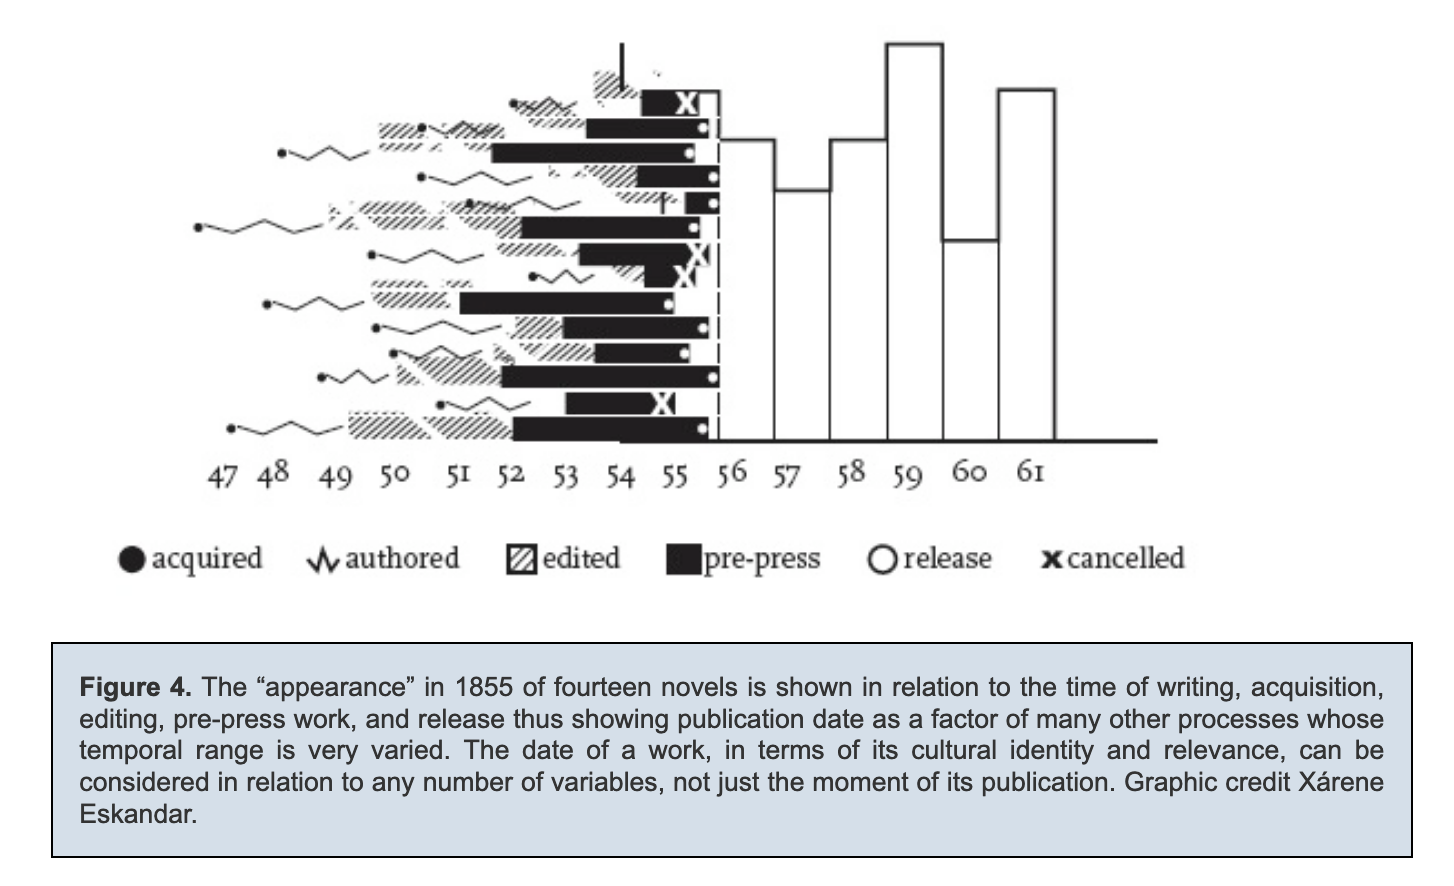
\includegraphics[width=.9\linewidth]{./img/Drucker.png}
\end{center}

Emphasizing "capta" is a way of figuring elements that have been
reduced, resolved, or ignored in traditional quantitative
analysis. Drucker makes evident what is overlooked or assumed when
dealing with complex subjects by muddling (rather than simplifying)
the relationship between elements.

In a certain sense, all of the above critics, Moretti, Da, Ramsay and
Drucker, rely on speculation in their criticism. First, there is
significant overlap between distant reading and speculative computing
in that they visualize or arrange textual data to stimulate
analysis. Moretti, after all, is using visualization to spark his
imagination and make conjectures, which he describes as
"explanations." In the pursuit of the falsifiable, Moretti evacuates
much of his method's creative potential. The difference is that
Moretti's Distant Reading uses makes conjectures within a falsifiable
framework. The difference between them, therefore, has to do with
their approach or orientation in using quantitative methods. Moretti
and Da show how computational methods encourage a "falsifiable" method
of literary criticism that mimics the methodologies of the
sciences. Alternatively, Ramsay and Drucker demonstrate how these
methods can also be used toward explicitly speculative ends, and for
Drucker in particular, with a sensitivity that is critical of
anlaytical processes.

The role of paranoia in distant reading blocks out other kinds of
connection to text. Moretti's method stems from a suspicious
conviction that the archive of literary history has something to
hide. Rita Felski explains that the desire in a “hermeneutics of
suspicion,” which she calls a militant mode of reading forecloses
possibilities of connection and being moved by these texts. Because
critics are focused on unearthing or discovering secrets in the text,
it reduces the interaction between reader and text to an intellectual
activity. Felski wonders what if we allowed ourselves to be marked or
struck by what we read. Then, rather than just be a cognitive
activity, reading can become an “embodied mode of attentiveness that
involves us in acts of sensing, perceiving, feeling, registering, and
engaging” (176). A critic like Stephen Ramsay, for example, is not
only willing to be surprised, his critical process is driven by a
desire for surprise. And Johanna Drucker, although not driven by
surprise, is searching for ways to disrupt assumptions about handling
and processing graphical data.


\subsection{II: the problem: queerness as untouchable}
\label{sec:org2764ec0}
\subsubsection{the untouchable and identity formation}
\label{sec:orgf5715b5}
The idea of the "untouchable" builds off queer theorists who have
isolated a queer experience of displacement, estrangement, or a
feeling of a lack that creates a space for emergent affects. This
experience derives from the political and social environment that
attempts to erase the existence of minorty subjects, particularly
queer people of color. Even as LGBT groups appear to gain more
visibily and acceptance, such gains are trapped within the limiting,
normative time of the present (citation to munoz). 

[expand this idea about normativization of queerness, with reference
to Bostock v. Clayton County---the major opinion bans discrimination
on the grounds of "sex discrimination"--i.e. queers have this
protection because straights have it. This is not expanding our
protection of desire to include queer forms of love, it is just
extending an antiquated view. The dissent by Alito is on the grounds
of "sex," which does not cover sexual orientation or gender ID, and by
Kavanaugh on the constraints of the court, who cannot legislate new
law but can only judge prior law. I agree with Alito \& Kavanaugh, as
they point to the pitfalls of heteronormativity, though I am happy
with the result.]

This chapter explores potential positions or orientations around
queerness. It begins by establishing queer subjectivity on the basis
of affect, and unpacks a core condition of queerness as "untouchable."
By "untouchable," I mean that queer identity is constituted through a
sensation of a lack, through the sensation of absence, contour,
boundary, edge, exclusion. This is opposed to majority
subject-formation, wherein "[t]he fiction of identity is one that is
accessed with relative ease" (Muñoz \emph{Disidentifications} 5). In what
follows, I locate "untouchability" in the affective experiences that
constitute subjectivity, experiences that isolate moments of
strangeness, disjunction, irony, ambivalence, and chaos. These
affective experiences center on a quality of incommensurability that
is the defining condition of untouchability [and will later become the
criterion of touching without touching]. This foundational quality of
the incommensurable, which makes queerness "untouchable," influences
our approach \emph{as critics} toward queer texts, themes, and
subjects. For queer readers in particular, there is a desire to
recognize within the past something that affirms queer experience in
the present, making acts of identification that collapse or overlook
the complexity of experience. Heather Love describes queer critics,
"Like demanding lovers [who] promise to rescue the past when in fact
they dream of being rescued themselves" (33). This chapter proposes a
reading method that enables queerness to be grasped, but at a
distance. The attention to affect provides the ground to remagine
reading as situated within the reader's embodied relationship to the
text.

\subsubsection{disidentification points to incommensurable affect}
\label{sec:org0570c01}
This chapter unpacks the condition of "the untouchable" from theories
of identity and communication developed by Queer Theorists from Latinx
backgrounds and traditions, including Muñoz, Ofelia Schutte, and
Gloria Anzaldúa. My approach toward subjectivity is based on a
paradigm of identity formation that Muñoz generalizes as
"identities-in-difference" (\emph{Disidentifications} 6). Muñoz's
identities-in-difference marshalls theories of difference from Chicanx
theorists Norma Alarcón's idea of "differential consciousness" and
Chela Sandova's concept of emergent identities-in-difference, which
center moments of failed interpellation as the core materials of
subject formation. Muñoz's work on identity offers a space for
prioritizing the role of affect in subject formation.

According to Muñoz, queer subjectivity grows from an affective
experience that he describes as "disidentification." Disidentification
describes how minority subjects negotiate identity in a cultural
sphere that disregards their existence. Due to "cultural logics of
heteronormativity, white supremacy, and misogyny," queer people of
color have been placed outside majority ideas about race, sexuality,
gender, and class, that constitute dominant society
(\emph{Disidentifications} 5). As a result, minority experience is defined
by a gap in identification, where subjectivity emerges in the failure
to adhere to social expectations. Within this gap, dominant
signfications of identity are not totally inaccessible to minority
subjects. Rather, they are accessed according to a process of
"disidentification," where subjects find alternative pathways of
connection to that which remains beyond their grasp. These moments are
fleeting sensations of finding oneself attracted to something that is
inappropriate, "\emph{to read onesself} and one's own life narrative in a
moment, object, or subject that is not culturally coded to 'connect'
with the disidentifying subject" (\emph{Disidentifications} 12; my
italics). Muñoz offers his own formative experience of
disidentification from a childhood memory of watching Truman Capote on
TV:

\begin{quote}
I remember, for instance, seeing an amazingly queeny Truman Capote
describe the work of fellow writer Jack Kerouac as not writing but,
instead, typing. I am certain that my pre-out consciousness was
completely terrified by the swishy spectacle of Capote's
performance. But I also remember feeling a deep pleasure in hearing
Capote make language, in "getting" the fantastic bitchiness of his
quip [\ldots{}] I can locate that experience of suburban spectatorship as
having a disidentificatory impact on me. Capote's performance was as
exhilarating as it was terrifying. \emph{Disidentifications} 4
\end{quote}

This memory is distinguished by a powerful disjunction between
opposite feelings, which consitutes identity from ambivalent
affects. The exhilaration that Muñoz feels when he understands
Capote's dig is compounded by the surprise of catching its "fanstastic
bitchiness." But this upheaval is attended by another feeling, a fear
of recognition, which is a foundational affect for queer
subjectivity. Kelly Caldwell, a poet and academic, explains in "The
Torment of Queer Literature" that "embracing queerness is often
embracing abjection" (par. 4). She describes her disidentificatory
experience reading James Baldwin's novel \emph{Giovanni's Room} as a
transgender woman, with "the risk of recognizing David’s denial and
repression as my own" (par. 17). Caldwell wonders, "what if the only
available act of identification is one of stigma and shame? [\ldots{}]
Sometimes identification is loss and despair" (par. 4). For Caldwell,
the process of "reading oneself\ldots{} in a moment, object, or subject
that is not culturally coded" is self-shattering.

In Muñoz's experience watching Capote, disidentification emerges in
the space between the opposing sensations of pleasure and terror. This
sensation of opposing affects and the shattering of identity has been
well explored by queer Chicana Theorist Gloria Anzaldúa. For Anzaldúa,
the figure of \emph{la mestiza}\footnote{Anzaldúa draws the figure of the \emph{mestiza}, or mixed woman,
from Mexican philosopher José Vasconcelos's promotion of "una raza
mestiza" [the mixed race].} denotes the experience of being
mixed, at the intersection of two opposing forces. The
mestiza----"[c]radled in one culture, sandwiched between two
cultures"---has the capacity to contain dualities, such as
male/female, English/Spanish, American/Mexican (78). Mestiza
consciousness is about hybridity, holding a tolerance for ambiguity,
for existing in the middle space that contains dualities. This
consciousness manifests in what Anzaldúa describes as the experience
of \emph{el choque}, or the shock: "The coming together of two
self-consistent but habitually incompatible frames of reference"
(78). The affective experience of \emph{el choque}," a cultural collision,"
consists of a bodily phenomenon where the subject receives multiple
opposing messages that incite a physical upheaval (78). The choque
occurs at the intersection of cultures, and also within culture:
"Through our mothers, the culture gave us mixed messages: \emph{No voy a
dejar que ningun pelado desgraciado maltrate a mis hijos}. And in the
next breath it would say, \emph{La-mujer tiene que hacer lo que le diga el
hombre}" (40). The clash of "mixed messages" results in mental and
emotional states of confusion and despair: "The mestiza's dual or
multiple personality is plagued by psychic restlessness" (78). It is
an embodied experience of physical and pyschic unsettlement that is a
basis for identity formation. 

The choque experienced in acts of queer disidentification points to a
core quality of queerness that is incommensurable. Latina feminist
philosopher Ofelia Schutte's modeling of cross-cultural
communication isolates a quality that is useful for understanding the
productive effects of the choque. Schutte, who draws from feminist
postcolonial and poststructuralist concepts of alterity and
difference, writes about communication between native English and
Spanish speakers. Her goal is to explore how subjects from different
cultures might achieve effective conversation, "to communicate with
'the other' who is culturally different from oneself"
(53). Communication begins with the assumption that "no two cultures
or languages can be perfectly transparent to each other" (56). There
is something lost in translation, "a residue of meaning that will not
be reached in cross-cultural endeavors" (56). This vestige of
communication that fails to transfer between subaltern and dominant
subjects is what she calls the incommensurable element. Schutte goes
into detail to explain how the incommensurable emerges in
conversation:

\begin{quote}
In cross-cultural communication, each speaker may "say" something that
falls on the side of the "unsaid" for a culturally differentiated
interlocutor. Such gaps in communication may cause one speaker's
discourse to appear incoherent or insufficiently organized. To the
culturally dominant speaker, the subaltern speaker's discourse may
appear to be a string of fragmented observations rather than a unified
whole. The actual problem may not be incoherence but the lack of
cultural translatability of the signifiers for coherence from one set
of cultural presuppositions to the other. 62
\end{quote}

The question of how to speak to those different from us allows one to
productively think through how queer subjects integrate their own
difference from society.

The point of isolating incommensurability is not to try to grasp or
translate the vestige of lost meaning, but to recognize that gap as a
space that constitutes subjectivity. We need to recongize this
incommensurability because it is a gap that opens up space for
emergent affects. Schutte's model emphasizes the productive effects of
attending to these gaps and ellisions. She encourages attention to the
ways in which "the other's speech, or some aspect of it, resonates in
me as a kind of strangeness, as a kind of displacement of the usual
expectation" (56). Schutte proposes that one embrace the strangeness
of communication, locating the moments where meaning seems to slip by
and elude us. By paying attention to the awkward and even bizarre
moments of misunderstanding, we find the materials for constructing
new dis(identity).

We are looking for alternative modes of analysis which allow us to
deal with the incommensurable elements of queerness.

\subsubsection{paranoia attempts to resolve incommens: sedgwick}
\label{sec:org0767671}

The goal here is to preserve the incommensurable in analysis. We want
to give full rein to the elements that escape and elude
understanding. We must first look at methods that attempt to resolve
incommensurability, and see how they reduce or flatten the complexity
of queer subjectivity \& experience.

The reality of incommensurability points to ways that understanding
will always be flawed, never complete, and never self-evident. The
illusion that we can gain sufficient understanding about queer
experience, that such experiences are "commensurable," drives certain
reading practices that critics describe as "paranoid" or "suspicious."
This reading practice assumes experience and subjectivity to be
fundamentally accessible. Here, the reading method pursues knowledge
as a goal in and of itself. To illustrate this effect, Eve Kosofsky
Sedgwick relates a conversation between herself and a friend during
few years of the AIDS crisis, when speculation about the government's
complicity in spreading the virus is rampant. At the time, Sedgwick
wonders whether "the lives of African Americans are worthless in the
eyes of the United States; that gay men and drug users are held cheap
where they aren't actively hated" (123). Her friend counters this
suspicion, pointing out that knowledge of conspiracy doesn't achieve
anything on its own: "Supposing we were ever sure of all those
things---what would we know then that we don't already know?"
(123). Merely knowing that something is true, revealing the presence
of systematic oppression, injustice, discrimination, does nothing. As
Sedgwick explains, knowledge of a problem is not enough to "enjoin
that person to any specific train of epistemological or narrative
consequences" (123).

Sedgwick explains that, "for all its vaunted suspicion, [paranoia]
acts as though its work would be accomplished if only it could
finally, this time, somehow get its story truly known"
(141). Moreover, a paranoid or suspicious stance blocks out other
possibilities for relation to the text.

Paranoid reading practices deliver results that are imaginable within
given knowledge structures.

\subsubsection{{\bfseries\sffamily TODO} clean replication, representation: haraway}
\label{sec:org58c48bb}

To examine the way that paranoid reading works, it is useful to
explore its workings in other disciplines. There is a lot we can learn
from history and science, in particular, about the ways that paranoid
reading collapses complexity and perpetuates established forms of
knowledge. Historicist literary scholar David Kazanjian explains how
the charge of "overreading," or the accusation that critics attribute
contemporary meaning to a historical text, presumes a strict
separation between historically contextualized reading and ahistorical
reading. Kazanjian points out that those who level this accusation
assume that so-called "historical" perspectives are accessible, "as if
one inhabited the same historical scene as the text one is reading"
("Scenes of Speculation," 80). Similar assumptions are made in
science, which in particular, demonstrate how paranoia enacts a
self-replicating mechanic. Though it appears in much of literary
studies, the impulse that drives paranoid reading is borrowed from a
critical viewpoint in scientific inquiry that assumes a detached
observer. Critiques of this position, particularly in Donna Haraway's
work on primatology, attempt to articulate a new mode of feminist
science that de-naturalizes the "natural." Haraway's research on
primates reveals the ways in which assumptions and preconceptions from
the (white, male) subject inflect the object of study. She examines
how scientists bring their own investments to bear even in the
seemingly benign questions they might ask, or qualities they isolate,
as areas of interest. For example, primatologists working with the
goal of studying social structures in the field often impose their own
social structures by turning their assumptions of male dominance into
"observations." Feminist scientists attempt to revise such narratives
by emphasizing organization and cooperation among primate communities:
"revisionists have stressed matrifocal groups, long-term social
cooperation rather than short-term spectacular aggression, flexible
process rather than strict structure” (19). Pointing out that, “Women
know very well that knowledge from the natural sciences has been used
in the interests of our domination and not our liberation," Harwaway
asserts that such revision is about empowering the subjugated,
reconceiving “female receptivity” as "female choice" (8). The creation
of a subject/object split \emph{reproduces} and legitimizes hierarchies of
domination.

Donna Haraway's words, a search for the "one code that translates all
meaning perfectly, the central dogma of phallogocentrism" (\emph{Simians,
Cyborgs, and Women} 176).

\subsubsection{{\bfseries\sffamily TODO} add Barad on replication / representationalism}
\label{sec:org3ceb61a}

Barad on representationalism. 

Joan Scott: the way that literary critics approach vision vs other
fields

Scott, Joan. “The Evidence of Experience”:
\begin{itemize}
\item Using experience for evidence rather than thinking about how
experience is shaped. Scott talks about representation, about
looking at experience, at the vision, the optical effects, for what
they suggest. The beautiful reading of Samuel Delany’s vision of the
“millions of gay men” the fantastical projection (rather than real
identity) that suggests a political consciousness. Historiography is
about modes of seeing.
\item Experience is always mediated for literary critics. We never take a
\end{itemize}
text as referential---there is rhetoric and form.

\subsubsection{{\bfseries\sffamily TODO} revise paranoia and recovery, hartman on limits of language}
\label{sec:org6381f8d}

Not only does paranoid inquiry tend to replicate the assumptions of
the observer, but it blocks out other forms of knowledge. This is
especially evident in the work of historical recovery, in the impulse
to find "hidden" or "forgotten" meaning in textual and archival
material. Recovery works by a self-legitimizing and perpetuating logic
that attempts to render what has been left out, disregarded, or
misunderstood within the logic of dominance. It is Jacques Derrida's
\emph{archive fever}, or the desire for legibility, under the auspices of
the ruler, which animates the endless search for origins. It is, in
Haraway's words, a search for the "one code that translates all
meaning perfectly, the central dogma of phallogocentrism" (\emph{Simians,
Cyborgs, and Women} 176).

The stakes of recovery work are uniquely stark in the history of the
Black Atlantic, where researchers must work to square the growth of an
inhuman practice within a historical narrative of progress and
liberalization. A tradition that rationalizes slavery with the right
to property, that justifies war through the social contract. Black
Atlantic scholars Lisa Lowe and Saidiya Hartman point out that the
central paradox of studying the archive of slavery is the structuring
condition of recovery. In her essay "History Hesitant," Lowe explains
that because recovery work necessarily occurs within the limits of the
authorizing power, it always subjects itself to that power. Rather
that work under these conditions, historians of enslaved experience
ought to examine this confining structure, "the archeology of
knowledge through which the archive subjects and governs precisely by
means of instruments that absent the humanity of the enslaved”
(87). Researchers might examine, for example, how "the slave trader’s
desire to record, measure, list, and account" weigh up against
"rationalist claims to produce truth or meaning about the terrors of
captivity, enslavement, or torture" (88). Saidiya Hartman similarly
turns to the question of epistemology as the crux of the recovery
work: “If it is no longer sufficient to expose the scandal, then how
might it be possible to generate a different set of descriptions from
this archive?" (7).

Oftentimes, new tools can obscure the ways that we replicate our own
assumptions. The advent of photography in the mid-nineteenth century
allowed subjects to codify their prejudices as science, for example,
in the pictures of American slaves taken by Louis Agassiz
in 1850. These daguerrotypes, a pioneering practice in photography
that uses light-sensitive chemicals on silver plates, show how the
impulse for scientific classification impacts the quality and kind of
knowledge that results. Agassiz, a Swiss anthropologist, came to the
United States to study the physical differences between European
whites and African blacks, by examining the shape and character of
their heads and torsos, similar to contemporary studies in physionomy
and phrenology that analyzed the exterior form of the human
body. Agassiz's goal was to amass evidence to support his theory, that
mankind had been separately created and whites and blacks were in fact
different species (Wallis 40). Using photography for anthropoligical
purposes, and organizing photographs to support a classification
system, Agassiz's work demonstrates how the apparent "objectivity" of
the photograph can mask the highly subjective motives for
classification. Writing about the photographs, which were exhibited by
the Amon Carter Museum in 1992, Brian Wallis explains that such images
were organized to suggest divisions between "self and other, healthy
and diseased, normal and pathological," with the insidious effect of
"mask[ing] its subjective distortions in the guise of logic and
organization" (Wallis 47, 54-55). The problem, Wallis points out, is
the realism of the photographic tool obscures the ways that subjects
harness it to solidify their preconceptions---"Strengthened by the
seeming transparency of photographic realism, these categories and the
divisions between them soon took on the authority of natural 'facts.'
Supplying either too much or too little information, photographs soon
muddied the easy distinctions between subjective knowledge and what
was called "objective." (47-48). The more seeminly transparent the
tool, the easier it is to wrangle it toward proving "self-evident"
truths.

In this case, the apparent fidelity of the photographic tool to record
"nature" in fact obscures the ways that using the tool only reinforces
a preconceived notion of "nature." Wallis explains that, "Supplying
either too much or too little information, photographs soon muddied
the easy distinctions between subjective knowledge and what was called
'objective' (48). The photographs reinforce the ways that scientific
tools, which appear to capture "reality," can be harnessed and
manipulated toward the observer's purpose.

Hartman's central problem is what to do with an absent archive. She
leaves us the paradox of recovery work: "How does one revisit the
scene of subjection without replicating the grammar of violence?"
(4). Hartman writes caustically about the impossibility of telling
stories that have been left out of the record. Not only that we can
never recover these stories (they are lost to time) but we can not
approximate them with our current tools, with language. In "Venus in
Two Acts," Hartman tells the story of Black Venus, the unnamed slave
woman who appears variously throughout the "offical" record:

\begin{quote}
we could have as easily encountered her in a ship’s ledger in the
tally of debits; or in an overseer’s journal—--“last night I laid with
Dido on the ground”; or as an amorous bed-fellow with a purse so
elastic “that it will contain the largest thing any gentleman can
present her with” in Harris’s List of Covent- Garden Ladies; or as the
paramour in the narrative of a mercenary soldier in Surinam; or as a
brothel owner in a traveler’s account of the prostitutes of Barbados;
or as a minor character in a nineteenth-century pornographic novel. 1
\end{quote}

[TODO a better close reading of the above block quote, what are the
figures here?]  

What draws all these iterations of Venus together is their silence,
"no one remembered her name or recorded the things she said, or
observed that she refused to say anything at all" (2). The fact of
silence cuts deeper than the failure of history but is part of the
condition known as the "violence of the archive," which denotes not
only absence as a form of evidence, in that the physical records are
missing, but also in the tools of expression, in language that cannot
approximate the reality of experience, and in the audible discourse
that dictates silence.

[end this section with a meditation on language not being enough. Now
I should then turn to the question of embodiment. The body will show
the way.]

\subsubsection{{\bfseries\sffamily TODO} cut/revise post-critical reading: sedgwick \& felski}
\label{sec:org29db3e8}
Just as we are limited by language, cannot approximate, we are also
stuck within the bodies of our thinking: emotion is inescapable in
criticism, whether it is suspicious or not. We are attached to what we
write about.

Let's approach this attachment as an opportunity. The fact that we
cannot be objective opens a window. 

\begin{enumerate}
\item Felski on the illusion of emotional detachment:
\label{sec:orgda33645}

The reality is that we are stuck in these bodies of our thinking. Rita
Felski describes how seemingly neutral and detatched critical stance
belies an emotional disposition:

\begin{quote}
Scholars like to think that their claims stand or fall on the merits
of their reasoning and the irresistible weight of their evidence, yet
they also adopt a low-key affective tone that can bolster or
drastically diminish their allure. Critical detachment, in this light,
is not an absence of mood but one manifestation of it---a certain
orientation toward one's subject, a way of making one's argument
matter. 6
\end{quote}

The "low-key affective tone" of scholarly discourse suggests that
affect, and the feeling subject associated with it, has been left out
of the critical process. However, appealing to the apparently
unemotional does not succeed in removing emotion from argument---this
is impossible---but it does reinforce the illusion that emotions don't
belong in rational thought. Actually they do---though the emotions of
critical discourse are of a quality and degree that mask their own
presence. Felski explains that, “Rather than an ascetic exercise in
demystification, suspicious reading turns out to be a style of thought
infused with a range of passions and pleasures, intense engagements
and eager commitments” (9). One follows the exposition of the framing
paradigms, the twists and turns of the driving question, the climax of
of discovery followed by the of denouement of the conclusion, one
immediately senses the full dramatic repertoire of critical
inquiry. 

\item Felski \& Sedgwick affective approaches
\label{sec:org4d411d5}

Critics like Rita Felski and Eve Sedgwick adopt an alternative
approach toward reading that exposes knowledge as derived from
embodied experience. Felski talks about reading as an affective
orientation, where readers position themselves and their desires
around texts. Felski critiques the popular orientation in literary
criticism centered on what Paul Riceour has called the “hermeneutics
of suspicion”---the desire to unmask and demystify the secrets of
literary works. According to Felski, critics generally behave as if
language is always withholding some truth, that the critic’s task is
to reveal the unsaid or repressed. She identifies the affective modes
of suspicion to include disenchantment, vigilance, paranoia. 

Sedgwick makes a similar assertion about tendencies of "paranoid
reading," though she bases her critique on Michele Foucault's
repressive hypothesis from his \emph{History of Sexuality, Vol. 1}, which
approaches discussions on sex and sexuality through the lense of
repression or prohibition. Rather than excavating the workings of the
repressive hypothesis, Foucault is interested in the ways that
discourse on sex has proliferated, in its multiplications that avoid
censure while satisfying the desire for sexual discourse. Left with no
place to go, discussion on sex simply continued to spread by
transforming itself into palatable discourses such as Marxism,
pyschoanalytic, libertarian, etc. By looking for the specter of
sex/power dynamics in these discourses, Foucault seems to work outside
the logic of the repressive hypothesis. But this is not the
case. Sedgwick explains that, "the almost delirious promise of the
book" is "the suggestion that there might be ways of thinking around
[the repressive hypothesis]" (9). In fact, Sedgwick explains that
Foucault's inquiry has been, from the start, structured by repression
and prohibition. She finds that the "critical analysis of repression
is itself inseparable from repression" (10). 

Felski and Sedgwick see a dead end in militant reading practices. 

Felski's nightmare: 
Sedgwick's wish: 

"How do we step outside the repressive hypothesis "to forms of thought
that would not be structured by the question of prohibition in the
first place?" (\emph{Touching Feeling} 11).

Speaking on Foucault's repressive hypothesis: "I knew what I wanted
from it: some ways of understanding human desire that might be quite
to the side of prohibition and repression, that might hence be
structured quite differently from the heroic, 'liberatory',
inescapably dualistic righteousness of hunting down and attacking
prohibition/repression in all its chameleonic guises" (\emph{Touching
Feeling} 10).

Felski shows how this suspicion toward texts forecloses other possible
readings while providing no guarantee of rigorous or radical
thought. Rather than adopt a suspicious attitude, Felski suggests that
literary scholars try “postcritical reading," which looks to what the
text suggests or makes possible. Felski wonders what if we allowed
ourselves to be marked or struck by what we read. Then, rather than
just be a cognitive activity, reading can become an “embodied mode of
attentiveness that involves us in acts of sensing, perceiving,
feeling, registering, and engaging” (176).

Reading is about movement 


Postcritical Reading --- "Reading, in this light, is a matter of
attaching, collating, negotiating, assembling—of forging links between
things that were previously unconnected”… “Reading, in this sense, is
not just a cognitive activity but an embodied mode of attentiveness
that involves us in acts of sensing, perceiving, feeling, registering,
and engaging” (Felski 176).

\item Sedgwick on generative shame
\label{sec:org3d1f85e}
What if we read Henry James mobilizing shame as a creative resource?
  For many queer people, shame is a structuring force in their
  identity. But this doesn’t mean we need to be negative, we can look
  to the ways that shame unlocks creativity and productivity---to the
  ways that metaphors are made possible through shame. James’
  “blushing”, “flushing” is linked to a fantasy of the skin being
  entered, or touched by a hand. GLOVE, GAGE, GAGEURE…  We can reclaim
  a negative affect of shame and approach it as a generative force.
\begin{itemize}
\item "Shame interests me politically, then, because it generates and
legitimates the place of identity--the question of identity--at the
origin of the impulse to the performative, but does so without
giving that identity space the standing of an essence. It
constitutes the as-to-be-constituted, which is also to say, as
already there for the (necessary, productive) misconstrual and
misrecognition. Shame--living, as it does, on and in the face--seems
to be uniquely contagious from one person to another. And the
contagiousness of shame is only facilitated by its anamorphic,
protean susceptibility to new expressive grammars" (63).
\end{itemize}
\end{enumerate}

\subsubsection{{\bfseries\sffamily TODO} revise hesitation, critical distance is necessary: Lowe}
\label{sec:org8d0a865}
-> To avoid paranoid methods we develop a critical distance, we turn to
the ways that "touch" can be distanced. 

Within the dominant culture, recovery means authorizing the structures
of knowledge that give rise to injustice in the first place. So what
do we do now? There are affects associated with this kind of
impasse. We hold ourselves back, restraint, avoidance. Lowe explains
that

\begin{quote}
Hesitation, rather than rushing to recover what has been
lost, need not be understood as inaction or postponement, or as a
thwarting of the wish to provide for a future world. Rather, it halts
the desire for recognition by the present social order and staves off
the compulsion to make visible within current epistemological
orthodoxy. 98
\end{quote}

Feelings of hesitation, doubt, dissapointment are ways of protecting
the archive of slavery from further exploitation.

To sum up: one solution to paranoid impulses involves is critical
awareness, the ability to access the affects that come between you and
the object of study. 

The archivist must work within the discrepancy between reality and the
historical record. Hartman's goal is "to expose and exploit the
incommensurability between the experience of the enslaved and the
fictions of history\ldots{} the requirements of narrative, the stuff of
subjects and plots and ends" (10).
\subsubsection{{\bfseries\sffamily TODO} refine \emph{feeling backward} as touching at a distance}
\label{sec:orgc3f6848}
--> Love offers a model of "feeling backward" which is a way for critics
to connect with queer subjects in a way that keeps objects out of the
critic's reach. 

Heather Love offers a reading strategy that acknowledges queer
experience, particularly suffering, as unconsoleable. In resisting the
temptations to redeem psychic suffering by queer subjects, Heather
Love offers a strategy called "feeling-backward." This strategy opens
a space for bad feelings without trying to recuscitate, justify, or
transform them. She focuses on feelings such as "nostalgia, regret,
shame, despair, \emph{ressentiment}, passivity escapism, self-hatred,
withdrawal, bitterness, defeatism, and loneliness," which, according
to Love, are tied to "the historical impossibility of same-sex desire"
(4, emphasis original). She examines the burdened protagonists from
famous modernist texts like Walter Pater's \emph{The Renaissance: Studies
in Art and Poetry} (1873), Radclyffe Hall's \emph{The Well of Loneliness}
(1928), Willa Cather's \emph{My Ántonia} (1918), and Sylvia Townsend
Warner's \emph{Summer Will Show} (1936). Love argues that the shame and
stigma experienced by these characters ought to be recognized rather
than resolved. Instead of turning negative histories into sites of
resistance or affirmation, these hurting characters might have full
reign over their own darkness. And this darkness must be where the
critic will meet them.

Love proposes a method in which the goal is not to redeem queer
subjects or resolve queer failure. Rather, the problem of
identification is turned to a reading strategy: "I want to suggest a
mode of historiography that recognizes the inevitability of a 'play of
recogniztions,' but that also sees these recognitions not as consoling
but as shattering" (45). Reading, for Love, can enact a "play of
recognitions," which is a way of making fleeting connections that do
not presume complete understanding. It is a way of identifying, but
not fully. Full identification would attempt to wrench the subject
from its suffering, and effectively transform it into something
else. Rather that attempt to rescusitate it, Love looks to the ways
that identity unsettles and dissolves subjectivity. She gives the
example of Stephen Gordon from Radclyffe Hall's \emph{The Well of
Loneliness}. Once considered too depressing as a model of lesbianism,
recent critics have cast Stephen Gordon as a transgender figure. Love
resists this label, maintaining that Stephen is “beyond the reach of
such redemptive narratives” (119). The question, for Love, is not
whether Stephen is a pre-op FTM (Female-to-Male), but how Stephen’s
existential negativity can be read as an embodied phenonmenon, as “a
social experience insistently internalized and corporeal” (108).



\begin{enumerate}
\item {\bfseries\sffamily TODO} organize queerness irrecoverable, but temptin g ID: Love
\label{sec:org76506d9}

The more hopeless and resistant queer subjects make for more tempting
identifications. Love explains how these subjects remain beyond the
reader's grasp: "As queer readers we tend to see ourselves as reaching
back toward isolated figures in the queer past in order to rescue or
save them. It is hard to know what to do with texts that resist our
advances" (8). The reason that these subjects remain so unreachable
has to do with the nature of queerness itself, which represents
absence, loss, and failure. Love illustrates this quality by evoking a
Greek myth, Orpheus and Eurydice, in which the lover botches his
beloved's rescue by looking back at her as they exit the
underworld. Love quotes from Maurice Blanchot's account of the story
in "The Gaze of Orpheus," to describe what Orpheus searches for in the
prohibited and doomed glance backward:

\begin{quote}
Not to look would be infidelity to the measureless, imprudent force
of his movement, which does not want Eurydice in her daytime truth and
in her everyday appeal, but wants her in her nocturnal obscurity, in
her distance, with her closed body and sealed face---wants to see her
not when she is visible, but when she is invisible, and not as the
intimacy of familiar life, but as the foreignness of what excludes all
intimacy, and wants, not to make her live, but to have living in her
the plenditude of death. 50
\end{quote}

Orpheus's downfall is his desire for a glimpse at what cannot be
grapsed, at what remains beyond the light. This desire is not for
"daytime truth" but for "noctural obscurity," which is always receding
at the moment of pursuit. Like Eurydice, queerness emerges only to
slip away, turning its face from the parched gaze. Can we be blamed
for looking for that which cannot be grasped? No, because queerness
has always been structured by that which is not, by what Love calls
"impossible love" (24). Not only is queerness projected to fail, it is
a project of failure. Love reminds us that "Queer history has been an
education in absence" (50). In learning failure and loss, queer
readers can only identify with what they have been taught to recognize
as untouchable. Full identification, like Eurydice in the daylight, is
prevented by design.

\item {\bfseries\sffamily TODO} organize the untouchable Queer, Butler \& Cvetkovitch
\label{sec:orgc07ee0f}
[here begin to write about Cvetkovitch on Stone Butch Blues, and/or
Butler on touching?]
\end{enumerate}


\subsection{III: solutions: abstraction, formalization, opacity}
\label{sec:org3e9192a}
Computational methods reveal an aesthetic of formalization as an
heuristic: just as text is transformed and manipulated into data, so
queerness is formalized into narrative and figurative
structures. Approaching queerness and computation as an aesthetic of
formalization opens a space where the rigidity of computational
methods and the fluidity of queer subjectivity intersect.

\begin{enumerate}
\item {\bfseries\sffamily TODO} add Munoz's point on the ecstatic, rounding out the point
\label{sec:orga26b924}
from the previous section on queerness as being "not yet here"
\end{enumerate}
\subsubsection{{\bfseries\sffamily TODO} refine reparative reading is active}
\label{sec:orgbbd4f73}

We might explore, with Sedgwick, "forms of thought that would not be
structured by the question of prohibition" (11). Sedgwick points that
that critical inquiry might work within a \emph{reparative} methodology,
which opens room for interpretive possibilities and attention to
positive affects like love, gratitude, and affection. This method
welcomes surprise of discovery over affirmation. It prioritizes "local
theories and nonce taxonomies" over totalizing perspectives (145). We
might approach criticism as having to do with \emph{movement} rather than
\emph{knowledge}:

\begin{quote}
[M]oving from the rather fixated question Is a particular piece of
knowledge true, and how can we know? to further questions: What does
knowledge \emph{do}---the pursuit of it, the having and exposing of it, the
receiving again of knowledge of what one already knows? How, in short,
is knowledge \emph{performative}, and how best does one move among its
causes and effects?" (my italics, 124)
\end{quote}

This reorienation of knowledge as \emph{active}, as performative, opens up
the critical process to one that is mobile and and speculative rather
than suspicious. Moreover, it draws attention to the ways that
knowledge is embodied, with all the surprises and discoveries that
embodiment entails. 
\subsubsection{{\bfseries\sffamily TODO} cut Waves on movement}
\label{sec:org2bb8774}
The narration works as a seduction by piquing the reader's interest in
the story, propelling her through hyperlinks across the various nodes,
and repeatedly frustrating her desire for closure or resolution.


The reader’s experience of frustration and desire in navigating
through the story mirrors the themes of sexual frustration and desire
within the story. The electronic format of the story is what allows
this theme to surface, for me. As I follow this disorienting
narrative, I similarly enter into cycles of desire and
frustration. This affective reaction is only possible through a
displacement---a formal displacement that uses electronic media to
re-organize, re-structure and display the story in the way we
encounter it.

Larry McCaffery, the fiction judge who awarded Fisher the ELO prize,
praises the hyperfiction’s use of fragmentation to present anecdotes,
bits of story and meditations in a way that liberates the story’s
potential: "Fisher creates an interconnected web of branching,
narrative possibilities" (“Comments”). Rather than feel paralyzed by
the variety of options, McCafferty regards such options as liberating
the traditionally pre-determined text into something more malleable,
and therefore, more relatable, to the reader. Jessica Laccetti also
lauds Waves’ indeterminate reading experience, saying that it cannot
have defined beginnings, section divisions, or endings. Each time the
reader sits down and opens this hypertext, it is different; depending
on the chosen order of node, the reader will derive new meaning from
that reading. She argues that, “as the narrative sequencing changes,
so does our understanding of reading” (180). By constantly rearranging
the order of its nodes, hyperfictions like Waves creates new, unique
narratives, “enabl[ing] numerous possibilities for beginnings and,
therefore, sequentialities” (Laccetti 180).

Roland Barthes offers a theory about the reader’s affective response
to the text that illuminates how hypertext may use linking as a
narrative strategy to engage, rather than dissuade, the reader. In The
Pleasure of the Text, Barthes describes two ways that texts provoke
reactions by appealing to the reader’s “readerly” or “writerly”
faculties. The text may stimulate pleasure or bliss in the reader
depending on the degree to which its language disrupts his reading
experience. On the one hand, the text of pleasure, or the “readerly”
text, is “the text that contents, fills, grants euphoria; the text
that comes from culture and does not break with it, is linked to a
comfortable practice of reading” (all italics original; 14).  The text
of bliss, the “writerly” text, on the other hand, is one “that imposes
a state of loss, the text that discomforts (perhaps to the point of a
certain boredom), unsettles the reader’s historical, cultural,
psychological assumptions, the consistency of his tastes, values,
memories, brings to a crisis his relation with language” (14). The
important difference here is the extent to which the text stimulates
affects that actively push the reader away or disrupt his reading. The
text of pleasure operates according to the principles of narrative
suspense that drive traditional stories, like cause and effect, while
the text of bliss negates these principles: “what pleasure wants is
the site of loss, the seam, the cut, the deflation, the dissolve which
seizes the subject in the midst of bliss” (Barthes 7). In other words,
the text of bliss is an interruption of the comfortable reading
experience that emphasizes the reader’s position as a
subject. According to Barthes, the text of bliss is a positive
experience for the reader insofar as he enjoys this interruption: “the
subject gains access to bliss by the cohabitation of languages working
side by side: the text… is a sanctioned babel” (4). Barthes
description here applies nicely to the structure of hypertext fiction,
in which different texts are embedded quite literally side by side in
the form of hyperlinks: insofar as the reader “sanctions” these texts,
he will experience them as texts of bliss.

 From its table of contents, the novella foregrounds the reader’s
agency in navigating through its fragmentary structure, where the
reader encounters a navigation page that lists eight main sections, or
chapters, of the narrative. These sections are named “kissing girls,”
“school tales,” “I want her,” “city,” “country,” “she was warned,”
“dare,” and “her collections.” When the reader pans over each chapter
title, a textual blurb appears containing an excerpt from that
chapter, which often draw from a sexual episode that stimulate
reader's interest in that chapter, enticing her onward. For example,
the excerpt for “I want her” presents an erotic moment between the
narrator and one of her lovers, Jennie.:

\begin{quote}
I’m in bed with Jennie Winchester and I realize she want me to undo
her pants. She needs to be home by 11:00 and needs to leave my place
by 10:45. I’m kissing her but opening my eyes at intervals to catch
the clock. At exactly 10:43 I unbutton her Levis and shove my hand
inside, barely undoing the zipper. “I’m in bed\ldots{}”
\end{quote}

The narrator severs the excerpt at a moment of climax, tempting the
reader to click through to the next node. Another section heading,
“dare,” displays a similar strategy: “Fay Devlin and I are playing
spin the bottle. She spins, but she trembles. By the time we get to
Truth or Dare, I have my lips on her nipple and I’ve made her do the
asking” (“These Waves of Girls…”). These excerpts establish the
reader’s agency and the novel’s fragmentary structure from the outset
of the novella. Because the chapters are unnumbered, the reader must
determine how to proceed through the sections of the novella by making
decisions about which to read first. These previews function to entice
the reader to click through to read the rest of that section. And
while the table of contents hints at the existence of an underlying
structure to the narrative, that structure also reveals itself to be
founded on fragments. In this way, the reader’s first encounter with
the text portends that she may never get the whole story, yet
encourages her onward.

In fact, as this semblance of narrative organization all but
disappears beyond the table of contents, it becomes increasingly clear
that the reader fully controls the order of nodes. After progressing
from the navigation page, the reader’s options multiply exponentially,
and these options compete for the reader’s selection. In order to
proceed through the text, the reader is forced to decide from the
abundance of choices. On this particular node, reached from the “I
want her” chapter title on the table of contents, hyperlinks run up
and down the left side of the screen and populate the main
text. Clicking through the first link in the main text, “Jennie,” the
reader reaches a node with nine links. Again, how does she choose to
proceed among these links? According to Barthes, the text of bliss
wants to be read: “the text you write must prove to me that it desires
me” (6). In deciding between the links that vie for her attention, the
reader may follow her own impulsivity (she may simply click on the
first link she sees, as she did on the previous page) or her interest
in the word being linked. The node tells a story about Jennie and
Tracey engaging in adolescent sexual exploits at summer camp. The
links on this page include “been to that campground,” “It's grade 10,”
“in my head I imagine a desperate love triangle,” “her hand under my
shirt,” “the s l o w movements of Jennie's fingers,” “a dyke -- I know
it -- but she won't do anything about it -- can't -- frozen,” “Close
the lights,” “We try not to move too much, too loudly,” and “attended
camp” (“Jennie only attended…”). At every node, the text proves again
and again that it desires her. The reader may decide to read through
this page, or read only a portion of the page, and interrupt her
progress to click on a link. Or the reader may forgo reading this page
altogether, and follow another link to a wholly new page. Either way,
she makes a decision in order to proceed, and her decision determines
the order of each node’s appearance. The text of bliss wants to be
read, and the reader must decide how. By assembling the node into a
specific order, the reader organizes the text of bliss according to
the unique path that she chooses.


Amin, Kadji, Amber Jamilla Musser, and Roy Pérez “Queer Form:
Aesthetics, Race, and the Violences of the Social” ASAP/Journal,
Volume 2, Number 2, May 2017, pp. 227-239: “Form informs queerness,
and queerness is best understood as a series of relations to form,
relations not limited to binary and adversarial models of resistance
and opposition” (228).

\subsubsection{{\bfseries\sffamily TODO} draft QPOC on opacity, recuperating absence}
\label{sec:org361c546}

"The critical challenge is to imagine a practice of archival reading
that incites relationships between the seductions of recovery and the
occlusions such retrieval mandates. By this I mean to say: What if the
recuperative gesture return us to a space of absence? How then does
one restore absence to itself? Put simply, can an empty archive also
be full?" (1). 

Hartmen's "critical fabulation"

The archivist must work within the discrepancy between reality and the
historical record. Hartman's goal is "to expose and exploit the
incommensurability between the experience of the enslaved and the
fictions of history\ldots{} the requirements of narrative, the stuff of
subjects and plots and ends" ("Venus" 10).
\begin{itemize}
\item "This double gesture can be described as straining against the
limits of the archive to write a cultural history of the captive,
and, at the same time, enacting the impossibility of representing
the lives of the captives precisely through the process of
narration" ("Venus" 11).
\end{itemize}

Amber Musser's surface aesthetics: POC theorists have shown us how
subjectivity is never quite attainable.

Amber Musser's "surface aesthetics": Reading the "surface" to present
a self that is plural and opaque, inaccessible and excessive.
\begin{itemize}
\item Writing on photographs of Billy Holiday. How these show a
"surfacea esthetics" that "highlights the mutability of the flesh
rather than interiority" (par. 11).
\item "we can understand surface as the underside of the
scientific/pornographic drive toward locating knowledge in an
“objective” image" (par. 2)
\end{itemize}

An image of Billy Holiday "shows us surface aesthetics in its emphasis
on shine" (par. 1).
\begin{itemize}
\item "many of the elements that shine—--pearls, eye shadow, and
lipstick--—decorate or cover Harris’s body. They alter its surface and
also make a spectacle of these superficial alterations. Taken
together these attributes emphasize the ways that surface hints at
the pleasures of opacity" (par. 2)
\item "Shine also complicates matters because of the way that it is
imbricated in representations of blackness\ldots{}Shine distracts from
the mandate of transparency and mobilizes hypervisibility—-the
cover of surface—-so that interiorities remain opaque\ldots{} so that
blackness is spectacular, but not knowable" (par. 3).
\item "these versions of self-portraiture go beyond mere representation
and mark \textbf{creative forms of expressivity that reveal forms of self
that exceed capture}\ldots{}The force of Billie \#21, then, emerges in
our recognition that the photograph is explicitly not revealing
Harris’s interiority, but that it instead illuminates the
possibility of reading Harris as a plural self both in relation to
Holiday through his performance of citation and in relation to the
otherness of himself that he summons" (par. 6)
\end{itemize}

Kazanjian, who works primarily with archival material, suggests that
"we learn to read for scenes of speculation" rather than description
(80).
\begin{itemize}
\item "All this suggests that the letter sounds its way toward making
sense of what Liberia has proven to be, a sounding that draws, no
doubt, on an oral and biblical literacy that was common among even
the least formally educated black settlers. Read for such formal and
textual elements, the letter offers us questions, asymmetries, and
open ends; it provides no punctual emancipation or definitive
return, but also no ultimate tragedy or decisive failure" (80).
\end{itemize}

\subsubsection{{\bfseries\sffamily TODO} add Confessions on opacity}
\label{sec:orgb6ef9b3}
Missing pages --- the marbled page substitutes speculation for recovery which the corporation wants (to monetize the image of “abnormal” genitalia). But the narrator didn’t want to include it. The absence of the picture doesn’t point to a physical absence, but to the inability to articulate exactly what was there according to the structures of the time.

This is like Klein's image of absence and Caughie's storm cloud, a refusal to engage with positivist impulse, but here it's taken to apply to alternative sexual identities. Some things, if already absent, are not meant to be “recovered”. They can just exist as an absence.

There are stakes in here about archival work and knowledge and what can and cannot be said. There is a massive gap in our understanding of transbodies and sex and it cannot be articulated or understood so it simply comes across as absent. The missing page creates an economy of speculation.

Relates to the inability of language to inform our understanding, because it becomes fixed---Caughie’s Storm Cloud. Rather than fix or recover, this give the reader an opportunity for imagination.

When they are trying to find a term for the way they are intimate: “I
don’t give language to things that are beyond it” (93). Things that are beyond language\ldots{} Language is a limitation, a delimitation. It is a circumscription.

\subsubsection{{\bfseries\sffamily TODO} revise invisibility is good, allows queers avoid being seen}
\label{sec:org288102c}

As disidentified, queer subjects remain outside of the confines of the
visible. To gain visibility within the dominant system only reproduces
visibility within the terms of that system. This position has been
articulated by critiques of feminism since the 70s and 80s, and later
on, in critiques of LGBT+ equality movements. bell hooks explains that
one of the main issues with the women's movement of the 70s and 80s
was a lack of agreement about the goals of feminism. Feminists that
advocate for "equality with men," miss the point of radical change
altogether: "As long as\ldots{} any group defines liberation as gaining
social equality with ruling class white men, they have a vested
interest in the continued exploitation and oppression of others"
(\emph{Feminist Theory} 15). By prioritizing equal rights, such as access
to employment, childcare, and social services, the women's movement
asks to be included in the existing system that is already oppressing
them. hooks is not saying that these aren't worthy or even necessary
causes, but that the changes enacted by such measures will not be
enough to raise the quality of life for oppressed and exploited
peoples. This in particular is harmful for black women, who, as women
of color, have the most to lose within the neoliberal ideology. hooks
asserts that "Feminism is a struggle to end sexist
oppression. Therefore, it is necessarily a struggle to eradicate the
ideology of domination that permeates Western culture on various
levels as well as a commitment to reorganizing society" (\emph{Feminist
Theory} 24). One of the major stakes in this chapter is to find ways
of subverting, resisting, or opting out of hegemonic understandings of
visibility as progress. This chapter will explore how being visible,
accessible, \emph{touchable} by the dominant power is being subjected to
the terms of that power. At that point, it will be clear that
queerness's status as untouchable works to enhance its political
potential.

\subsubsection{{\bfseries\sffamily TODO} draft Toward a Queer Form}
\label{sec:orge26772b}
Writing the self is connected to form. Always. The form is
multiple. The form makes subjectivity opaque, but in the act of
abstraction, making it opaque, we can touch it and play around with
it. 

Opacity as value (Amin, Musser)

“For our purposes, queer form means challenging the primacy of the
visual, which has too often been a site for pernicious power
relations… At their base, such operations of surveillance and
classification rely on the concept of immutable difference, on sharp
boundaries, and on the possibility of exhaustively knowing the
other…. We see queer form as an aesthetics that moves persistently
around the visual, thereby avoiding this flattening. To the extent
that form operates behind the scenes as ideological impulse and
materiality, queer formal practices can resist the dictates of
transparency normally required of non-normative subjects by
illuminating the unseen. In this way it not only troubles the
epistemic assurances of the visual regime, but it also asks how
shifting away from static visuality can circumnavigate questions of
objectification. A move toward the diffusely sensual, and away from
the linearity of visual gazing, articulates difference in terms that
are not about dominance or norms, but that underscore the importance
of thinking with other modes of knowing, theorizing, and
experiencing. Queer form is about other ways of understanding
relationships to power and relationships to being” (Amin, Musser,
Perez 232-3)

Form understood as associated with queerness, queer experience, and as a way to disrupt easy understanding. Form can be queer and queer form can be opaque: 
“Form informs queerness, and queerness is best understood as a series of relations to form, relations not limited to binary and adversarial models of resistance and opposition” (228).
“Queer form” emerges… as a name for the range of formal, aesthetic, and sensuous strategies that make difference a little less knowable, visible, and digestible. This special issue makes a case for the value of indirection, opacity, and withholding as queer strategies for minoritarian art producers” (235).
 “form focuses attention on how violence—homophobia, racism, gentrification, capitalism, and colonialism, for instance—has structured conditions of possibility in material and epistemological ways” (232).
touch as an intersection for queerness and DH, both highly sensual
in that they abstract from the source

\subsubsection{{\bfseries\sffamily TODO} draft Butler on movement/contact/touch}
\label{sec:orgbde1bae}
\subsubsection{{\bfseries\sffamily TODO} draft the dimensions of touch: anzaldua}
\label{sec:orgdfeaae2}
--> the challenge is to regain touch without resolving it--overcoming
impulse of subj/obj divides. how do we touch without presuming full
connections? the answer is through abstraction, formalization,
opacity\ldots{}

Touch reconciles the inherent connection between bodies, something
that heteronormativity tries to suppress. For things to not touch, to
be severed or "objectified," moves them into a relation of
violence. Gloria Anzaldua explains that separation is brutal: "In
trying to become 'objective,' Western culture made 'objects' of things
and people when it distanced itself from them, thereby losing 'touch'
with them. This dichotomy is the root of all violence" (37). Losing
touch is a prerequisite for exploitation. The sundering of "objects"
from our touch primes us to take advantage of them. Colonial history
is a case study in losing touch: "White America has only attended to
the body of the earth in order to exploit it, never to succor it or to
be nurtured in it" (68). Anzaldua's \emph{mestiza}, birthed in the open
wound of the border, "where the Third World grates against the first
and bleeds," is an attempt to bring together what has been separated
(3). Those who live on the border know better than anyone--divisions
between bodies puts those bodies into conflict.

Touch offers myriad ways of relation. Eve Kosofsky Sedgwick offers
touch as a way of connecting to objects that evades "dualistic
thought," that is, in "binary" thought, where things are presumed to
be discrete and opposed. 

"But it is not enough to stand on the opposite river bank, shouting
questions,. challenging patriarchal, white conventions.  A
counterstance locks one into a duel of oppressor and oppressed; locked
in mortal ,combat, like the cop and the criminal, both are reduced to
a common denominator of violence\ldots{} At some point, on our way to a new
consciousness, we will have to leave the opposite bank, the split
between the two mortal combatants somehow healed so that we are on
both shores at once and, at once, see through serpent and eagle eyes"
(Anzaldúa 78-79 in old book).

Confronting the incommensurable requires subjects to step temporarily
into the place of the other, "that person or experience which makes it
possible for the self to recognize its own limited horizons in the
light of asymmetrically given relations marked by sexual, social,
cultural, or other differences" (Schutte 54).

This physical upheaval is the ground from which the mestiza builds
identity: "The new mestiza copes by developing a tolerance for
contradictions, a tolerance for ambiguity. She learns to be an Indian
in Mexican culture, to be Mexican from an Anglo point of view. She
learns to juggle cultures" (79).

As Cherríe Moraga points out, "it is not really difference the
oppressor fears so much as similarity" (La Guera, 30). Although the
feeling of incommensurability is central to queer experience, it can
be accessible to majority groups. Getting in touch with the \emph{choque},
however, is a great challenge for minority subjects, and an even
greater challenge for those of dominant cultures. For those who can
avoid it, there is an aversion to confront the "stranger within."

In short, for queer bodies, there is a dual impulse, a desire to touch
and be touched that coexists with the inability for touch to satisfy,
provide redemption, or avoid violation. Respecting the right not to be
touched, some queer theorists pursue critical methods that prevent
overidentification or overanalysis. They resist reading practices,
which have been called "suspicious reading" or "paranoid
reading"\footnote{Rita Felski? and Eve Kosofsky Sedgwick.\label{org40c1da5}}, that seek to expose the effects of homophobic
prohibition and repression with the goal of affirming queer subjects
or recuperating their losses. Paranoid or suspicious reading is
oriented around finding and exposing the pain and shame of the closet
in order to turn them into sites of political resistance, liberation,
or pride.

This leads us to the main problem with touch: it goes both ways. What
I touch also touches me; one body impressed by or in collision with
another. Eve Kosofsky Sedgwick explains that "the sense of touch makes
nonsense out of any dualistic understanding of agency and passivity;
to touch is always already to reach out, to fondle, to heft, to tap,
or to enfold" (13). Touch engages a range of relations where power is
not always reduced to opposition. The sensation of touch often
obscures this dual effect. Some bodies appear to desire touching
rather than being touched; sometimes, the desire for touch does not
seek contact, but the fullness of desiring.  it is bidirectional,
reveals a subject/object divide.

\subsubsection{{\bfseries\sffamily TODO} draft Frontera on vitality}
\label{sec:orge5d2414}

the book as living and structured
\begin{quote}
In looking at this book that I’m almost finished writing, I see a
mosaic pattern (Aztec-like) emerging, a weaving pattern, thin here,
thick there. I see a preoccupation with the deep structure, the
underlying structure, with the gesso underpainting that is red earth,
black earth. I can see the deep structure, the scaffolding. If I can
get the bone structure right, then putting flesh on it proceeds
without too many hitches. The problem is that the bones often do not
exist prior to the flesh, but are shaped after a vague and broad
shadow of its form is discerned or uncovered during beginning, middle
and final stages of the writing. Numerous overlays of paint, rough
surfaces, smooth surfaces make me realize l am preoccupied with
texture as well. Too, I see the barely contained color threatening to
spill over the boundaries of the object it represents and into other
"objects" and over the borders of the frame. I see a hybridization of
metaphor, different species of ideas popping up here, popping up
there, full of variations and seeming contradictions, though I believe
in an ordered, structured universe where all phenomena are
interrelated and imbued with spirit. This almost finished product
seems an assemblage, a montage, a beaded work with several leitmotifs
and with a central core, now appearing, now disappearing in a crazy
dance. The whole thing has had a mind of its own, escaping me and
insisting on putting together the pieces of its own puzzle with
minimal direction hom my will. It is a rebellious, willful entity, a
precocious girl-child forced to grow up too quickly, rough,
unyielding, with pieces of feather sticking out here and there, fur,
twigs, clay. My child, but not for much longer. This female being is
angry, sad, joyful, is Coatlicue, dove, horse, serpent, cactus. Though
it is a flawed thing---a clumsy, complex, groping blind thing---for me
it is alive, infused with spirit. I talk to it; it talks to me. (66-67
\& 88-89)
\end{quote}




\subsection{Vantanges/Opacity}
\label{sec:orge4ee3e8}

\subsubsection{Klein, Mandell, Caughie, Gaboury}
\label{sec:org7eb255d}
[Klein and D'Ignazio on the impossibility of neutral visualizations]
And the illusion of reason as being devoid of emotion is not limited
to verbal discourse. It also pervades--perhaps even more
insidiously---the apparently objective reprsentations data
visualization. Graphs, charts, and maps all contain persuasive
elements that succeed through their invisibility, in the trust, for
example, that the souces are truthfully represented in the
visualization or the implied preference of some metrics over
others. Lauren Klein and Catherine D'Ignazio point out that "so-called
'neutral' visualizations that do not appear to have an editorial
hand\ldots{} might even be the most perniciously persuasive visualizations
of all!" (\emph{Data Feminism}, chapter 2). Not dots on a graph can be said
to be removed from the predelictions of the creator and the generosity
of the viewer.

\subsubsection{Interweave with Saidiya Hartmann?}
\label{sec:org5fa005d}
\subsubsection{Against totalization}
\label{sec:orga131cf0}
\subsubsection{The visible and the invisible, opting out}
\label{sec:org6ea0854}





\subsection{MISC}
\label{sec:org967703e}

\begin{enumerate}
\item homonormativity: add supreme court decision
\label{sec:org60ee219}
[Queerness is being wrenched within heteronormative agendas----IE the
2020 surpreme court decision that protects queer desire bc it protects
straight desire].

\item queerness as estrangment
\label{sec:orgf23d180}
Arondekar, A., Cvetkovich, A., Hanhardt, CB, Kunzel, R., Nyong’O, T.,
Rodríguez, JM, \& Stryker, S. (2015). Queering archives: A roundtable
discussion. Radical History Review, 2015(122),
211-232. \url{http://dx.doi.org/10.1215/01636545-2849630} Retrieved from
\url{https://escholarship.org/uc/item/7z19h7rg}

This roundtable discusses the "archival turn" in queer studies, and
questions the methods, subjects, investments of queer archival
studies. 

Tavia Nyong'O: "I have never really deviated from the formative
impression Foucault gave that what I should expect from the archive is
the estrangement of myself and others, or that I could call that
estrangement queer" (216).
\end{enumerate}

\subsubsection{Clement, Bode, recent applications of deformance}
\label{sec:orgc96511f}

More recently, textual scholars have taken McGann's influential ideas
about Deformative Criticism and used them to study the ways that texts
are transformed in the process of digitization. Katherine Bode, for
example, engages McGann's ideas about deformance with theoretical
physics in working with electronic text. Bode explains that attention
to the "apparatus," or the instrument of analysis, allows her to
trouble the traditional subject/object binary between researcher and
text to examine "how\ldots{} we inscribe the boundaries we often presume to
represent" ("Data Beyond Representation" par 11). Drawing from a
theoretical physics understanding, where "an apparatus is a specific
material configuration, including of physicists, wherein certain
properties become determinate, while others are excluded," Bode
applies the figure of the apparatus to literary databases (Bode "Data
Beyond Representation, par. 24). Bode offers an example with her
current project, \emph{Reading at the Interface}, which explores the ways
that Australian literature has been characterized in literary
databases by various "paratexts," or "writings about literature"
("Data Beyond Representation" par 11). Bode looks at how the process
of data collection for these databases makes a distinction between the
main text and the "paratext," which includes metadata like title,
author, and publication information of the text. The project explores
how paratexts across various platforms, including academic journals,
newspapers, \emph{Goodreads}, and \emph{Librarything} have represented the
boundary of "Australian Literature," literally creating the boundary
of what we understand to be "text" and "paratext" in Australian
literature. Bode explains that she's "not interested in representing
discussion of 'Australian literature' on Goodreads so much as in
materialising that platform in ways that cannot be separated from
[the] categories of analysis" ("Data Beyond Representation"
par. 19). This activity reveals, for Bode, how the researcher (via the
"apparatus") intevenes with the object of analysis.

Applying McGann's ideas about deformative criticism to sound studies,
Tanya Clement explores how deformance enables embodied interactions
with text. In a project on visualization, she uses the audio analysis
tool "ProseVis" to visualize the prosodic elements of Gertrude Stein's
poetry, which creates dynamic spaces for the reader to interact with
the visualization. Using ProseVis, the reader can navigate through the
visualizations and manipulate the metrics for analysis. Clement points
out that just as a musical score "is read, but it is also meant to be
played, to be spatialized in time and embodied by voices (or
instruments) within a certain physical and hermeneutical context," the
same can be true for quantitative visualizations of text: "One 'reads'
a visualization, but to 'play' the visualisation is to engage the
spatialized interpretation of that visualisation as an embodied reader
in a situated context within a specific hermeneutical framework
("Distant Listening" par. 10). From this project, Clement theorizes
critical analysis as "play," where the critic "performs" the work just
as musicians might interpret a musical score, by "creat[ing] another
level of abstraction with which the interpreter engages" ("Distant
Listening par. 7). According to Clement, the multiple levels of
abstraction for containing the "work" of the text multiply the levels
of engagement with that text.

The unique affordance of digital environments, according to McGann,
Bode and Clement, is that they allow for numerable interventions upon
the textual object. The above authors approach computation as an
opportunity to examine the material specificities of eletronic
formats.

\subsubsection{Altschuler and Weimar on reproducibility}
\label{sec:orgab382d8}

--> reproducing something perfectly overlooks the ways that all
digital objects are unique, differentiated. Theory of textual
criticism which shows how ther are more interesting things to do then
create a digital "copy texte". 

This notion extends to digital humanist practitioners. 

they call to overturn the "unproblematic translatability of
information between the senses" while maintaining that reproduction is
the highest value. They argue to "texture the humanities", pointing
out that much of DH prioritizes the visual over other senses --
"privilege sight as the sense through which knowledge is accessible"
(74). Rightly so, they argue, “The textured DH we call for here
acknowledges that we cannot study knowledge only abstractly, apart
from the senses, and that we cannot study literature, art, and history
without including the history of embodied experiences” (74-75).
\begin{itemize}
\item “Touch This Page! uses 3-D printed facsimiles of raised-letter text
to inspire reflection on the assumptions most people make about
which senses are involved in reading” (82).
\end{itemize}

But they elide the one interesting trajectory when they place
reproduction over remediation/deformance. They state their aims: “to
expand the sensory accessibility of archives for all users and to do
so through the digital reproduction---rather than the translation---of
tactile knowledge” (76). Case example of the perfect reproduction:
\begin{itemize}
\item A scenario where “users\ldots{} can download a visual copy with
\end{itemize}
descriptive data, engage with the text in virtual reality, and create
their own textured facsimile. This technology once more makes possible
the tactile reading experiences for which this volume was designed and
promises library patrons a richer engagement with touch than most
archives can currently provide---even in person (85-86). 

The use case scenario makes the assumption that a reproduction is the
ideal form of textuality, despite their asserted aims for "diversity
of embodied experiences":
\begin{itemize}
\item “we must avoid tilting after the fiction of some ideal digital
surrogate---like a virtual reality system that would flawlessly
mimic original objects---lest we become digital Pierre Menards,
expending extensive energy to improve our reproductions to discover,
at last, that only the original perfects represents itself… Instead,
we envision in our tactile futures multiple strategies that could
not only open up access to varied experiences---past and
present---but also diversity the ways embodied experiences structure
our digital worlds” (86).
\item in order to open up “multiple strategies” and diversity embodied
experiences, we need a theory of text that is capacious enough to
accept variation and transmediation.
\item This argument overlooks deformance is a solution: the ways that
creating new texts, paratexts, creates new objects of knowledge. It
overlooks the performative, ala McGann, Clement.
\end{itemize}

In this view, digital becomes a means of optimization, efficiency,
total knowledge and understanding.
\subsubsection{Defining queer, Amin on historicizing through affect}
\label{sec:orgc41f1d3}
queerness manifests as an affective relation between the
subject and desired object. Kadji Amin defines queer as "fundamentally
affective\ldots{} a matter of sensing a resonance between one's object of
study and the inchoate cluster of feelings that inhabit and animate
the term queer" (173).
\subsubsection{Reading touching: within our bodies}
\label{sec:orgf3d40e3}
This point bears repeating---we are always stuck within the bodies of
our thinking. As such, we might as well turn to ourselves, to explore
(rather than how things are in the world) how things are \emph{to
us}. Sedgwick points out that the problem is not one of knowledge, but
one of movement. We can try to in-\emph{corporate}, as much as possible,
alternative reading methods that get at the unique experience of being
a thinking/feeling human that is fiddling with these tools. We can, in
other words, examine the possibilities of \emph{touching} what we read. And
we can do so with digital tools for text analysis and machine
learning.  However, there still exists a view that distant reading
lacks the sensitivity of close reading. "Critics who want to
sensitively describe the merits of a single work usually have no need
for statistics" (xxi).

\subsubsection{data reduction / queer assimilation}
\label{sec:orga8bdec9}
For those that would argue that negative feelings are no longer
relevant in today's world, Heather Love responds that the advent of
assimilation, of popular acceptance, only creates more problems for a
group that has come into being as abject. \emph{(the corrolary for digital
studies is the proliferation of data, of information, digitization)}
Queer assimilation and apparent rise in acceptance across popular
culture and mass media contradicts the reality of shame and stigma
that everyday queers experience, a contradiction that breeds ever more
shame: "Of course, same-sex desire is not as impossible as it used to
be; as a result, the survival of feelings such as shame, isolation,
and self-hatred into the post-Stonewall era is often the occasion for
further feelings of shame. The embarrassment of owning such feelings,
out of place as they are in a movement that takes pride as its
watchword, is acute" (4). What do we do with these residual feelings
of shame?

How should queer criticism orient itself? Love shows that critics face
a contradiction, brought on by the reality of negative feelings and
psychic costs of being queer in a homophobic society. The narrative
trajectory of queer progress runs counter to the residual pain of
being queer. Criticism is stuck in the middle of this ambivalence,
between affirming its pride and bemoaning its suffering: "We are not
sure if we should explore the link between homosexuality and loss, or
set about proving that it does not exist" (Love 3).

\subsubsection{Critique of affirmation: Cvetkovitch}
\label{sec:org806bbc4}

Attempts to affirm negative queer experience can be harmful. Ann
Cvetkovitch's work on trauma studies provides an example of how this
tendency can create further misunderstanding about suffering. In her
book, \emph{Archive of Feelings}, Cvetkovitch explores expressions of
trauma within the public sphere. She asks how individuals might
reclaim some of the most negative and traumatic feelings into
something positive and theraputic: "I want to place moments of extreme
trauma alongside moments of everyday emotional distress that are often
the only sign that trauma's effects are still being felt” (3). She
wrests trauma studies out of medical discourse and into public
culture---turning something that is traditionally private and
pathologized into something communitarian, an open, everyday "archive
of feelings."

Importantly, Cvetkovitch marshalls this reconfiguration of trauma to
expand what we consider the 'archive'. She also makes some incisive
points about the inability to fully portray suffering: "Because trauma
can be unspeakable and unrepresentable and because it is marked by
forgetting and dissociation, it often seems to leave behind no records
at all" (7). Cvetkovitch explores alternative methods of figuring
trauma, which are transformed when they enter the public sphere. She
cites examples from public performances like rock shows or
documentaries, in which the artists enact "moments of intense affect
that are transformative or revealing” (26). 

Although her focus on the affective and ephemeral dimension of
performance opens up conceptions of the archive, Cvetkovitch perhaps
goes too far when she suggests that these performances are redemptive
or in some way compensate for traumatic experience. She indicates that
such performances go so far as to alleviate psychological damage and
suffering: “Imaginative work that may bear an oblique relation to the
actual event of sexual abuse can ultimately be more ‘healing’ than an
explicit rendering of the event” (94). Trauma is a real medical
condition, with real consequences (death) for those who do not seek
treatment or downplay its life-threatening effects. Critics should be
careful in extending a definition of trauma that will end up hurting
those who are affected by it. We do not need to move trauma strictly
from the medical discourse in order to have a more communitarian,
open, and public relationship to it. There are other ways to confront
stigma which doesn’t attempt to redeem it, as Love explores with her
notion of “Feeling Backward.”

The step that Cvetkovitch takes with regard to trauma is interesting,
however, for what it suggests about the role of the critic in
analysis. The point isn't to find evidence of overcoming queer
suffering, but to examine the ways that queerness is figured in
abstraction. What does queerness look like, what can it do? 

\subsubsection{Munoz's disidentification quotes}
\label{sec:org388a987}

"We desire it but we desire it with a difference"
(\emph{Disidentifications} 15).

"Disidentification is about recycling and rethinking encoded
meaning. The process of disidentification scrambles and reconstructs
the encoded message of a cultural text in a fashion that both exposes
the encoded message's universalizing and exlusionary machinations and
recircuits its workings to account for, include, and empower minority
identities and identifications. Thus disidentification is a step
further than cracking open the code of the majority: it proceeds to
use this code as raw material for representing a disempowered politics
or positionality that has been rendered unthinkable by dominant
culture" (\emph{Disidentifications} 31).

"The chapters that make up this study attempt to chart the ways
in which identity is enacted by minority subjects who must work
with/resist the conditions of (im)possibility that dominant culture
generates. The cultural performers I am considering in this book must
negotiate between a fixed identity disposition and the socially
encoded roles that are available for such subjects"
(\emph{Disidentifications} 6). 

\subsubsection{Misc Quotes}
\label{sec:org8159fd3}
"how might activating emotion – leveraging it, rather than resisting
emotion in data visualization – help us learn, remember, and
communicate with data?" (Klein and D'Ignazio, \emph{Data Feminism},
chapter 2)

\subsubsection{\emph{Voyant-Tools}}
\label{sec:orgd7d6d8c}
Jerome McGann "prosthetic extensions"
Potential texts: Woolf's \emph{Orlando}. 

\begin{itemize}
\item Interweave a narrative about touch. Taking new materialist ideas but
\end{itemize}
placing them within context of QPOC critiqe. Anzaldua and Bennet on
touch and severing. Sarah Ahmed too. 

\subsubsection{\emph{These Waves of Girls}}
\label{sec:org548794c}
Following narrative desire. The click of the mouse allows readers to
move with the text, based on their own paths. 

\subsubsection{what are some print texts that enact these principles of movement?}
\label{sec:org0fcbd21}
\begin{itemize}
\item Alison Bechdel's "Are You My Mother": where every page is vibrating
\end{itemize}
with reference. 

\subsubsection{What, do you imagine that I would take so much trouble and so much}
\label{sec:org40dbdde}
pleasure in writing, do you think that I would keep so persistently to my task, if I were not preparing — with a rather shaky hand — a labyrinth into which I can venture, in which I can move my discourse, opening up underground passages, forcing it to go far from itself, finding overhangs that reduce and deform its itinerary, in which I can lose myself and appear at last to eyes that I will never have to meet again. I am no doubt not the only one who writes in order to have no face. Do not ask who I am and do not ask me to remain the same: leave it to our bureaucrats and our police to see that our papers are in order. At least spare us their morality when we write.’
\begin{itemize}
\item Michel Foucault, \emph{Archaeology of Knowledge}, 17.
\end{itemize}

\subsubsection{Kadji Amin, Amber Jamilla Musser, and Roy Pérez explain that paranoid}
\label{sec:org7307a08}
impulses "rely on the concept of immutable difference, on sharp
boundaries, and on the possibility of exhaustively knowing the other"
(232).

\subsubsection{The debates about TEI illustrates this tension between the}
\label{sec:org46dd19d}
“conservative” and the “creative” impulses in textual editing, and
shows how an encoding method that is highly structured can be used to
mark or explore moments of textual instability or ambiguity.

\subsubsection{felski on affects beside suspicion}
\label{sec:org12ba222}



Postcritical Reading…  “in this sense, is not just a cognitive
activity but an embodied mode of attentiveness that involves us in
acts of sensing, perceiving, feeling, registering, and engaging”
(Felski 176). 

Felski: At stake is our receptivity: “to allow ourselves to be marked,
struck, impressed by what we read” (Felski 12). 

"the reader-text connection becomes part of a network rather than a
self-enclosed dyad— yet a connection that remains vital to literary
studies, especially in the classroom. Reading, in this light, is a
matter of attaching, collating, negotiating, assembling—of forging
links between things that were previously unconnected. It is not a
question of plumbing depths or tracing surfaces… Interpretation
becomes a coproduction between actors that brings new things to light
rather than an endless rumination on a text’s hidden meanings or
representational failures” (Felski 174)

Surface reading challenges that search for absence by compelling a
reader to stay with what the text says and how it says it rather than
moving ahead to probe how it reflects and refracts larger cultural
patterns. This critique reifies aesthetic objects and suggests that
literary critics should embrace the literary.

\subsubsection{mcpherson, benjamin on race and tech}
\label{sec:orgd8f310a}
Major developments in technology also perpetuate racial
assumptions. Moving from networking technologies to software
development, Tara McPherson explores the parallels between the
Operating Systems and race relations, to show how the development of
computer software betrays hegemonic assumptions about whiteness and
elisions of difference.\textsuperscript{\ref{org40c1da5}} She focuses on the key moment of 1960s
United States, when Operating Systems, which is the foundational
software that supports a computer's programs and basic functioning,
developed alongside civil rights discourses. Her research focuses on
how "the organization of information and capital" in OS development
resonates in the struggles for racial justice: "Many of these shifts
were enacted in the name of liberalism, aimed at distancing the overt
racism of the past even as they contained and cordoned off progressive
radicalism" (30). McPherson deconstructs the UNIX operating system
which includes a hierarchical file system, a command line interpreter
(the Terminal on Mac or Command Prompt on Windows), and a variety of
software programs that are designed to work in tandem. McPherson
points out that UNIX-based Operating Systems (like Mac and Linux) are
distinguished by the ways that they partition and simplify complex
processes into discrete components, similar to the ways that identity
politics cordones off parts of the (social and technological) system
into distinct units. While this cordoning was productive for the
promotion of civil rights, it also, according to McPherson, "curtailed
and short-circuited more radical forms of political praxis, reducing
struggle to fairly discrete parameters" (30).

Crystallizing the intersection between Operating Systems and race
relations, McPherson asserts that "Certain modes of racial visibility
and knowing coincide or dovetail with specific ways of organizing
data" (24). McPherson emphasizes the "rules" of UNIX philosophy, which
lay out how UNIX's development prioritized the organization and
simplification of data processing:
\begin{quote}
Rule of Simplicity: Design for simplicity; add complexity only where
you must. Rule of Parsimony: Write a big program only when it is clear
by demonstration that nothing else will do. Rule of Transparency:
Design for visibility to make inspection and debugging easier\ldots{} Rule
of Representation: Fold knowledge into data so program logic can be
stupid and robust. 26
\end{quote}
The rules of "Simplicity" and "Parsimony" ensure that programs will be
composed of small, interlocking parts that can be easily updated and
transported to newer versions. The rule of "Transparency" flattens
nuance and ambiguity, making program components as legible as
possible. The rule of "Representation," particularly the suggestion to
"Fold knowledge into data" reduces the complexity of raw data, so that
it can be easily input into multiple processes. According to
McPherson, all of these rules work together to shore up the central
design theory of "modularity,"\footnote{DEFINITION NOT FOUND.} which stipulates that components
are self-contained and interoperable, so they can be independently
created, modified, and replaced without affecting the whole system.

The role of control in creating the internet and the emphasis on data
reduction in developing operating stystems leave their legacies on
21st century digital technology, where race becomes collapsed into
data. Echoing McPherson, Ruha Benjamin asserts that technology
reproduces social inequities under the guise of objectivity and
progressivism.\footnote{DEFINITION NOT FOUND.} Turning to technology, Benjamin explores how
innovations in Artificial Intelligence and algorithmic computing
extend racist paradigms into ever new tools, particularly in data
gathering and surveillance. The creators of these new technologies
mark, track, and quantify blackness, for example, in databases for
healthcare or financial services that associate "black names" with
criminality (Benjamin 5). With each update, technology is continually
promoted as efficient and progressive in a way that masks how it
exploits data about its subjects. Benjamin explains, "we are told that
how tech sees “difference” is a more objective reflection of reality
than if a mere human produced the same results\ldots{} bias enters through
the backdoor of design optimization in which the humans who create the
algorithms are hidden from view" (5-6). As she points out, "the road
to inequity is paved with technical fixes” (7). Like the creators of
UNIX, the creators of such tools and algorithms operate under
assumptions of white universality that inevitably marks blackness as
"other."

\subsubsection{sedgwick on liberatory vs prohibition}
\label{sec:org82a8b2b}
Sedgwick searches for "some ways of understanding human desire that might
be quite to the side of prohibition and repression, that might hence
be structured quite differently from the heroic, 'liberatory,'
inescapably dualistic righteousness of hunting down and attacking
prohibition/repression in all its chameleonic guises" (10).


\section{commands}
\label{sec:orgf772323}
c-c c-x f => create a new footnote
c-u c-c c-x f then select s => renumber footnotes

block quotes: \#+BEGIN\(_{\text{QUOTE}}\) \& \#+END\(_{\text{QUOTE}}\)
\end{document}
